\documentclass[a4paper,11pt]{article}
\usepackage{charter}
\usepackage[english]{babel}
\usepackage{graphicx, float, varioref, array, mathtools, enumitem, url}
\usepackage{amsmath, amssymb}
\usepackage[a4paper,margin=2cm]{geometry}
\usepackage{booktabs}
\setlist{noitemsep, topsep=0pt}

% ─── Title-page helper ────────────────────────────────────────────────────────
\usepackage{titling}
\usepackage{xcolor}

\begin{document}

% ═════════════════════════════════════════════════════════════════════════════
%  TITLE PAGE
% ═════════════════════════════════════════════════════════════════════════════
\begin{titlepage}
\centering
\vspace*{1.5cm}

% Institution block
{\Large\bfseries Danmarks Tekniske Universitet}\\[4pt]
{\large 02225 Distributed Real-Time Systems}\\[2pt]
{\normalsize Mini-Project 1 \textbar{} Group 1}

\vspace{1.2cm}
\noindent\rule{\linewidth}{0.8pt}
\vspace{0.4cm}

{\huge\bfseries Schedulability and Worst-Case Response Time\\[8pt]
               Analysis of Periodic Real-Time Tasks\\[8pt]
               under DM and EDF}

\vspace{0.4cm}
\noindent\rule{\linewidth}{0.8pt}

\vspace{1.5cm}

\begin{tabular}{ll}
\textit{Authors}                     & \textit{Student number} \\[6pt]
Andreas Bruun                        & s214955 \\
Pruthvi Bhat                         & s260070 \\
Kar\'{i}tas \'{O}sk P\'{a}lmad\'{o}ttir & s175414 \\
Kadambini Peri                       & s243438 \\
Akash Ravichandran                   & s250154 \\
\end{tabular}

\vspace{2cm}
{\normalsize Date: 20/02/2026 -- 11/05/2026}

\end{titlepage}

% ─────────────────────────────────────────────────────────────────────────────
\section{Introduction}
% ─────────────────────────────────────────────────────────────────────────────

Real-time systems must satisfy strict timing constraints: every task must complete before its
deadline, regardless of system load. For periodic tasks on a uniprocessor, two algorithms are
widely studied. \emph{Deadline Monotonic} (DM) scheduling is a fixed-priority, offline scheme
that assigns the highest priority to the task with the shortest relative deadline---optimal
among all fixed-priority schedulers for constrained-deadline sets~\cite{buttazzo2024}.
\emph{Earliest Deadline First} (EDF) is a dynamic-priority, online scheme that always executes
the ready task whose absolute deadline is closest---optimal overall on a single processor.

The central practical difference between the two is their utilisation ceiling. EDF is
schedulable if and only if the total CPU utilisation $U = \sum C_i/T_i \leq 1$, whereas DM
provides no tight closed-form utilisation bound: a set with $U$ well above the sufficient
hyperbolic bound can still pass DM (via exact Response-Time Analysis), but certain task
parameter combinations will fail DM while EDF succeeds.

This report compares DM and EDF across four utilisation levels---30\%, 50\%, 70\%, and
90\%---using 80 synthetic task sets of 10 tasks each. For each set we compute:
\begin{enumerate}
    \item DM Worst-Case Response Times (WCRTs) via Response-Time Analysis (RTA, Buttazzo
          \S4.5.2);
    \item EDF schedulability via the Processor Demand Criterion (PDC, Buttazzo \S4.6.1);
    \item EDF WCRTs via an exact event-driven hyperperiod simulation where the hyperperiod is
          tractable; and
    \item observed response-time statistics from a 300-run Monte Carlo stochastic simulation
          with execution times drawn uniformly from $[\text{BCET}, \text{WCET}]$.
\end{enumerate}

Section~\ref{sec:methodology} describes the task model and analysis methods.
Section~\ref{sec:results} presents the schedulability and WCRT results.
Section~\ref{sec:discussion} interprets the findings.
Sections~\ref{sec:conclusion} and~\ref{sec:limitations} summarise conclusions and future
directions.

% ─────────────────────────────────────────────────────────────────────────────
\section{Methodology}
\label{sec:methodology}
% ─────────────────────────────────────────────────────────────────────────────

\subsection{Task Model}

We model $n$ synchronous, periodic, constrained-deadline tasks
$\{\tau_1, \ldots, \tau_n\}$ on a single processor. Each task $\tau_i$ has:
\begin{itemize}
    \item $C_i$ (WCET): worst-case execution time, used for all analytical calculations.
    \item $B_i$ (BCET): best-case execution time, $B_i \leq C_i$, used in the stochastic simulation.
    \item $T_i$: period (inter-release time).
    \item $D_i$: relative deadline, with $D_i \leq T_i$ (constrained deadlines).
\end{itemize}
CPU utilisation is $U_i = C_i / T_i$ per task and $U = \sum_{i} U_i$ in total. All task sets use
a synchronous release model (all tasks first released at $t = 0$) on a single core ($P = 1$),
with $n = 10$ tasks per set, 20 sets per utilisation level, and 4 levels (u30, u50, u70, u90),
giving 80 sets in total.

\subsection{Deadline Monotonic Analysis (RTA)}
\label{sec:dm}

DM assigns priorities statically: the shortest relative deadline receives rank 0 (highest
priority), with ties broken by shorter period. Schedulability is determined by
\emph{Response-Time Analysis}~\cite{buttazzo2024}, the necessary and sufficient test for
fixed-priority preemptive scheduling. For each task $\tau_i$ (processed in
highest-to-lowest priority order), the WCRT $R_i$ is the fixed point of:
\begin{equation}
    R_i^{(k+1)} = C_i + \sum_{j \in \mathrm{hp}(i)} \left\lceil \frac{R_i^{(k)}}{T_j}
    \right\rceil C_j, \qquad R_i^{(0)} = C_i
    \label{eq:rta}
\end{equation}
where $\mathrm{hp}(i)$ is the set of tasks with strictly higher priority than $\tau_i$.
The term $\lceil R_i/T_j \rceil \cdot C_j$ is the maximum interference from $\tau_j$
during any busy window of length $R_i$. Iteration continues until $R_i^{(k+1)} = R_i^{(k)}$
(convergence, WCRT found) or $R_i^{(k)} > D_i$ (early exit, infeasible). Task $\tau_i$
is schedulable iff $R_i \leq D_i$.

\subsection{EDF Schedulability: Processor Demand Criterion}
\label{sec:edf_sched}

EDF is optimal for uniprocessor scheduling: a task set is EDF-schedulable iff it is
schedulable by any algorithm. For synchronous constrained-deadline sets the Processor
Demand Criterion~\cite{buttazzo2024} gives a necessary and sufficient test:
\begin{equation}
    U \leq 1 \quad \text{and} \quad \forall\, t \in (0, H]:\;
    \mathrm{dbf}(0,t) \leq t
    \label{eq:pdc}
\end{equation}
where $H = \mathrm{lcm}(T_1,\ldots,T_n)$ is the hyperperiod and the Demand Bound Function is:
\begin{equation}
    \mathrm{dbf}(0,t) = \sum_{i=1}^{n} \max\!\left(0,\,
    \left\lfloor \frac{t + T_i - D_i}{T_i} \right\rfloor\right) C_i
\end{equation}
Since $\mathrm{dbf}$ is piecewise constant, only scheduling points
$t = k T_i + D_i$ (absolute job deadlines, for $k = 0, 1, \ldots$, while $t \leq H$) need
to be checked. For $U < 1$ any violation must appear within the finite critical busy period
$\sum C_i / (1 - U)$, so the check terminates quickly regardless of hyperperiod size.

\subsection{EDF WCRT: Exact Hyperperiod Simulation}
\label{sec:edf_wcrt}

For a synchronous task set where every job executes for exactly its WCET, the EDF schedule
is deterministic and periodic with period $H$. The exact per-task WCRT is therefore obtained
by simulating the preemptive EDF schedule over $[0, H)$:
\begin{enumerate}
    \item Generate all jobs: $\tau_{i,k}$ releases at $r_{i,k} = k T_i$ with absolute
          deadline $d_{i,k} = r_{i,k} + D_i$, for $k = 0, 1, \ldots$ while $k T_i < H$.
    \item Simulate via an event-driven min-heap (priority = earliest absolute deadline).
    \item Record finish time $f_{i,k}$ for each job; response time $R_{i,k} = f_{i,k} - r_{i,k}$.
    \item $\mathrm{WCRT}_i = \max_k R_{i,k}$.
\end{enumerate}
Non-harmonic task periods can produce hyperperiods whose total job count
$\sum_i H/T_i$ reaches tens of billions. The simulation is therefore skipped for sets
where this count exceeds 200\,000 jobs. The PDC schedulability check is always performed,
but exact EDF WCRTs are reported only where the simulation is feasible.

\subsection{Harmonic Task-Set Benchmark}
\label{sec:harmonic_method}

To address the hyperperiod explosion identified in the primary benchmark, a second set of
80 task sets was generated with \emph{harmonic} periods: each task's period is chosen as
a power-of-two multiple of a common base, guaranteeing
$H = \mathrm{lcm}(T_1,\ldots,T_n) \ll \prod T_i$.
The same four utilisation levels (u30, u50, u70, u90) and the same 20-sets-per-level
structure were used (seed = 42, $n = 10$ tasks per set), so results are directly comparable
with the primary benchmark. By construction, every harmonic set has a total job count
$\sum_i H/T_i \leq 200\,000$, making exact EDF WCRT simulation feasible for all 80 sets.
The same DM RTA, EDF PDC, and 300-run Monte Carlo pipeline was applied unchanged.

\subsection{Stochastic Monte Carlo Simulation}
\label{sec:sim}

To compare analytical bounds with observed behaviour, each tractable task set is simulated
300 times with randomised execution times. In each run, every job $\tau_{i,k}$ is assigned
an execution time drawn uniformly from $[B_i, C_i]$, and the preemptive EDF schedule is
simulated over $[0, H)$. Per-task statistics recorded are: observed maximum response time,
mean, 95th percentile (P95), and 99th percentile (P99). The deadline miss rate (fraction of
runs with at least one missed deadline) is also recorded. Task sets exceeding 200\,000 jobs
are excluded from the stochastic simulation for the same reason as above.

% ─────────────────────────────────────────────────────────────────────────────
\section{Results}
\label{sec:results}
% ─────────────────────────────────────────────────────────────────────────────

\subsection{Schedulability Rates}

Table~\ref{tab:schedulability} summarises the schedulability results across all 80 task sets.
DM and EDF both achieve 100\% at utilisation levels 30\%, 50\%, and 70\%. At 90\% utilisation,
EDF continues to schedule all 20 sets, while DM fails on 2 (taskset-12, $U = 0.900$;
taskset-13, $U = 0.897$). Overall, DM schedules 78/80 sets (97.5\%) and EDF schedules 80/80
(100.0\%).

\begin{table}[H]
\centering
\caption{Schedulability results per utilisation level (20 sets each, $n = 10$ tasks/set, 300 sim.\ runs).}
\label{tab:schedulability}
\begin{tabular}{lrrrr}
\toprule
Level & Target $U$ & Actual $U$ range & DM pass rate & EDF pass rate \\
\midrule
u30   & 0.30 & 0.297--0.310 & 20/20 (100\%) & 20/20 (100\%) \\
u50   & 0.50 & 0.493--0.512 & 20/20 (100\%) & 20/20 (100\%) \\
u70   & 0.70 & 0.690--0.712 & 20/20 (100\%) & 20/20 (100\%) \\
u90   & 0.90 & 0.895--0.908 & 18/20~~(90\%) & 20/20 (100\%) \\
\midrule
Total & --   & 0.297--0.908 & 78/80~~(97.5\%) & 80/80 (100.0\%) \\
\bottomrule
\end{tabular}
\end{table}

Figure~\ref{fig:sched_vs_util} shows the results as a grouped bar chart. The divergence
between DM and EDF is visible only at the highest utilisation level tested.

\begin{figure}[H]
\centering

\includegraphics[width=0.72\textwidth]{figures/schedulability_vs_utilization.png}
\caption{Schedulability rate (\%) for DM and EDF at each utilisation level (20 sets per group).
         EDF maintains 100\% across all levels; DM drops to 90\% at $U \approx 0.90$.}
\label{fig:sched_vs_util}
\end{figure}

\subsection{WCRT Comparison: DM versus EDF}

Figures~\ref{fig:wcrt_u30}--\ref{fig:wcrt_u90} show the per-task WCRTs under DM and EDF
for one representative set at each utilisation level, with the relative deadline shown as a
stepped red line. Under DM, lower-priority tasks (longer deadlines) accumulate interference
from all higher-priority tasks via Eq.~\eqref{eq:rta}, producing steeply rising WCRTs.
Under EDF, priorities shift dynamically so interference is spread more evenly, yielding
substantially lower WCRTs for the lower-priority tasks---often well below their deadlines.
In the two DM-fail cases at u90, the WCRT of at least one task exceeded its deadline; EDF
passed both sets ($U \leq 1$, demand bound satisfied).

\begin{figure}[H]
\centering
\begin{minipage}{0.48\textwidth}
    \centering
    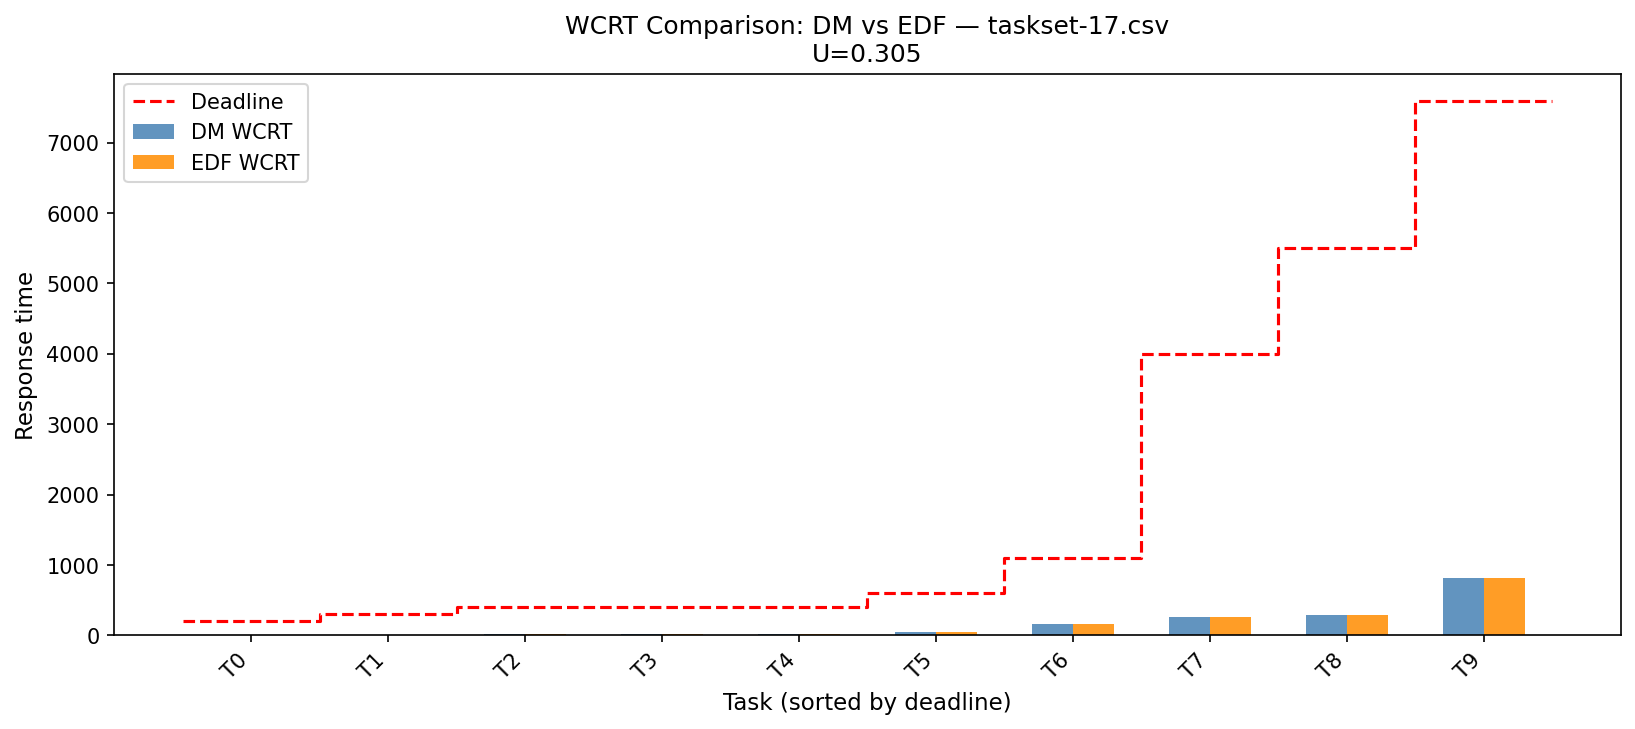
\includegraphics[width=\textwidth]{figures/wcrt_u30_taskset-17.png}
    \caption{WCRT: DM vs.\ EDF at $U \approx 0.30$ (taskset-17).}
    \label{fig:wcrt_u30}
\end{minipage}\hfill
\begin{minipage}{0.48\textwidth}
    \centering
    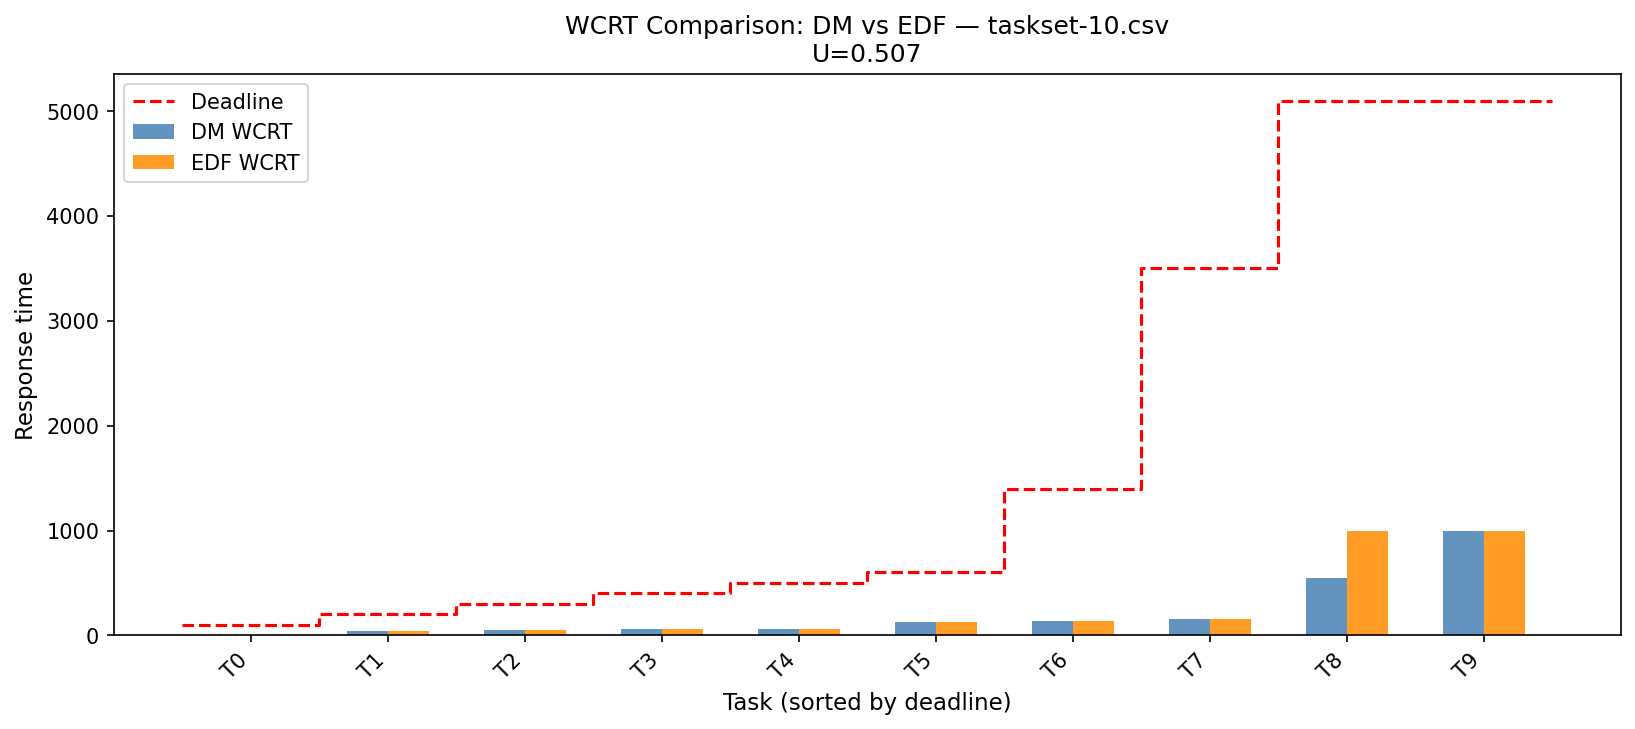
\includegraphics[width=\textwidth]{figures/wcrt_u50_taskset-10.png}
    \caption{WCRT: DM vs.\ EDF at $U \approx 0.50$ (taskset-10).}
    \label{fig:wcrt_u50}
\end{minipage}
\end{figure}

\begin{figure}[H]
\centering
\begin{minipage}{0.48\textwidth}
    \centering
    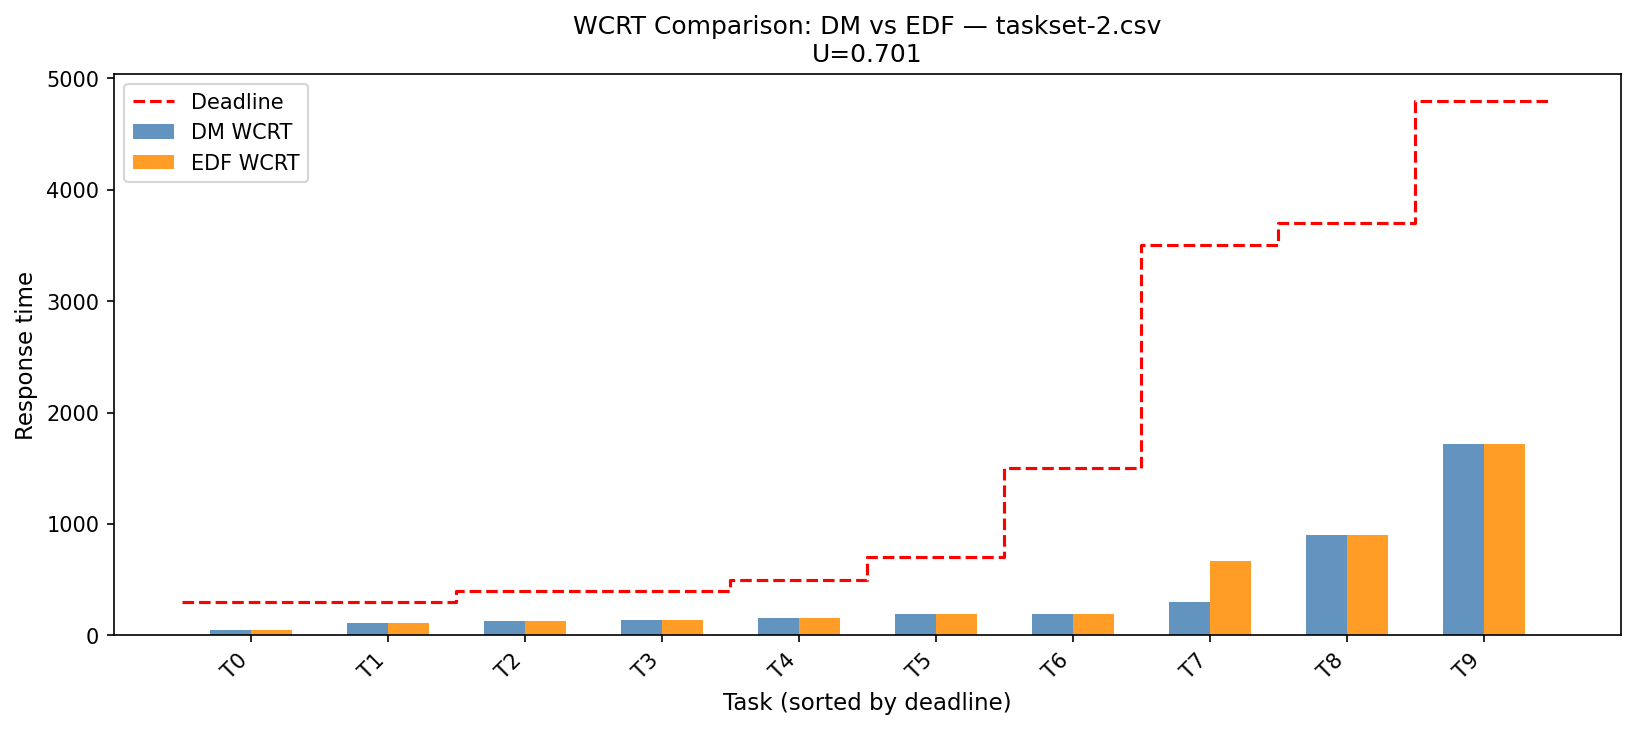
\includegraphics[width=\textwidth]{figures/wcrt_u70_taskset-2.png}
    \caption{WCRT: DM vs.\ EDF at $U \approx 0.70$ (taskset-2).}
    \label{fig:wcrt_u70}
\end{minipage}\hfill
\begin{minipage}{0.48\textwidth}
    \centering
    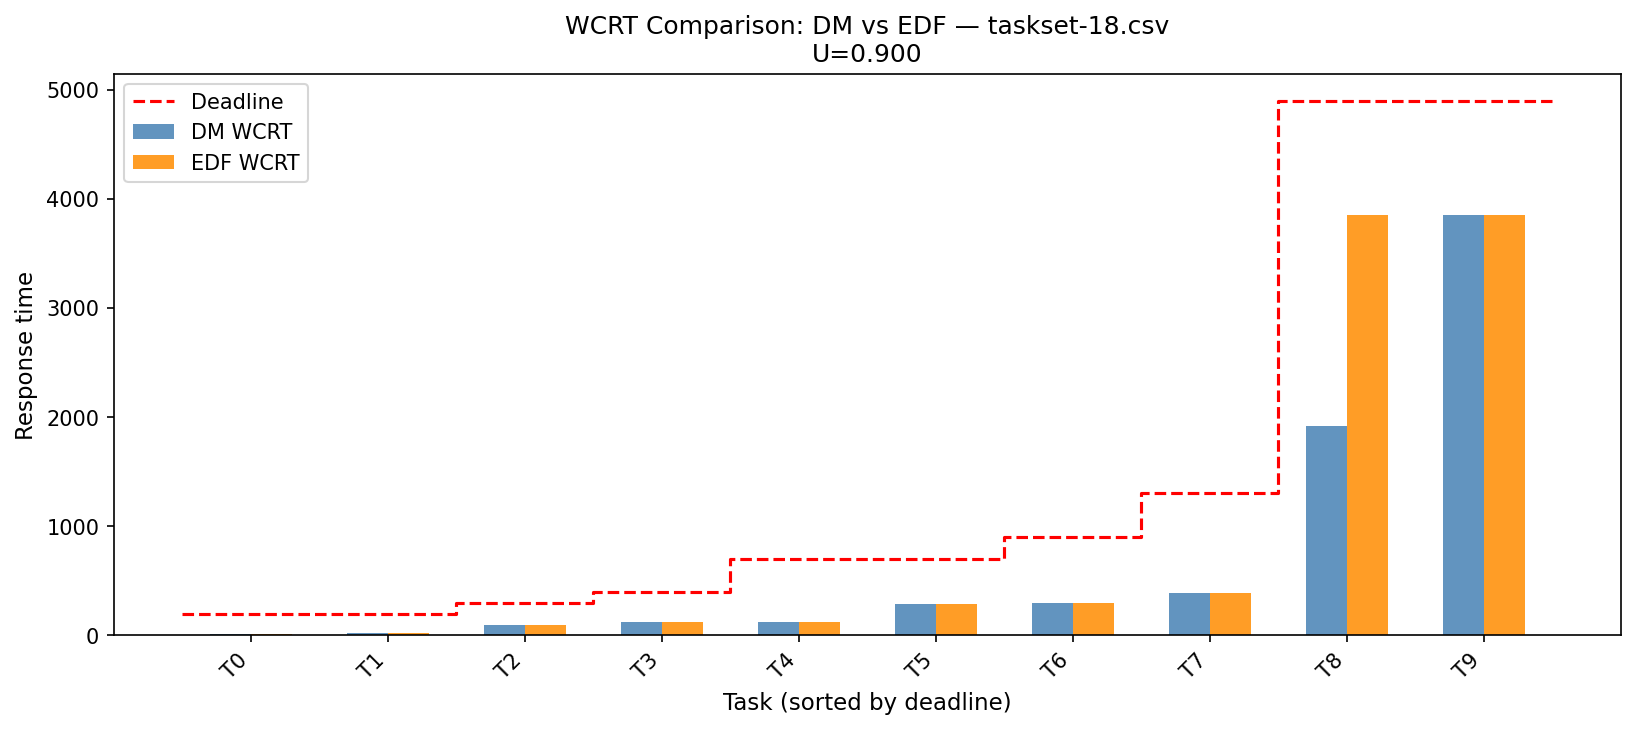
\includegraphics[width=\textwidth]{figures/wcrt_u90_taskset-18.png}
    \caption{WCRT: DM vs.\ EDF at $U \approx 0.90$ (taskset-18, DM passes).}
    \label{fig:wcrt_u90}
\end{minipage}
\end{figure}

\subsection{Analytical Bounds versus Simulated Response Times}

The majority of task sets (66 of 80) have non-harmonic periods that produce hyperperiods with
more than 200\,000 jobs, making exact EDF simulation infeasible. For the remaining 14 sets
where simulation ran, the stochastic Monte Carlo produced zero deadline misses (miss rate
0.0\%) across all 300 runs and all sets.

Figures~\ref{fig:cdf_u30}--\ref{fig:cdf_u90} show the empirical CDF of observed response
times for one representative set per utilisation level. In every plot:
\begin{itemize}
    \item The analytical EDF WCRT (red dashed) lies strictly to the right of all observed
          values, confirming the bound is valid.
    \item The mean response time (green dash-dot) is substantially lower than the WCRT,
          illustrating the pessimism inherent to worst-case analysis.
    \item P95 and P99 (visible from the CDF) cluster near the mean, not the WCRT, indicating
          that the worst-case alignment of job releases occurs extremely rarely in practice.
\end{itemize}

\begin{figure}[H]
\centering
\begin{minipage}{0.48\textwidth}
    \centering
    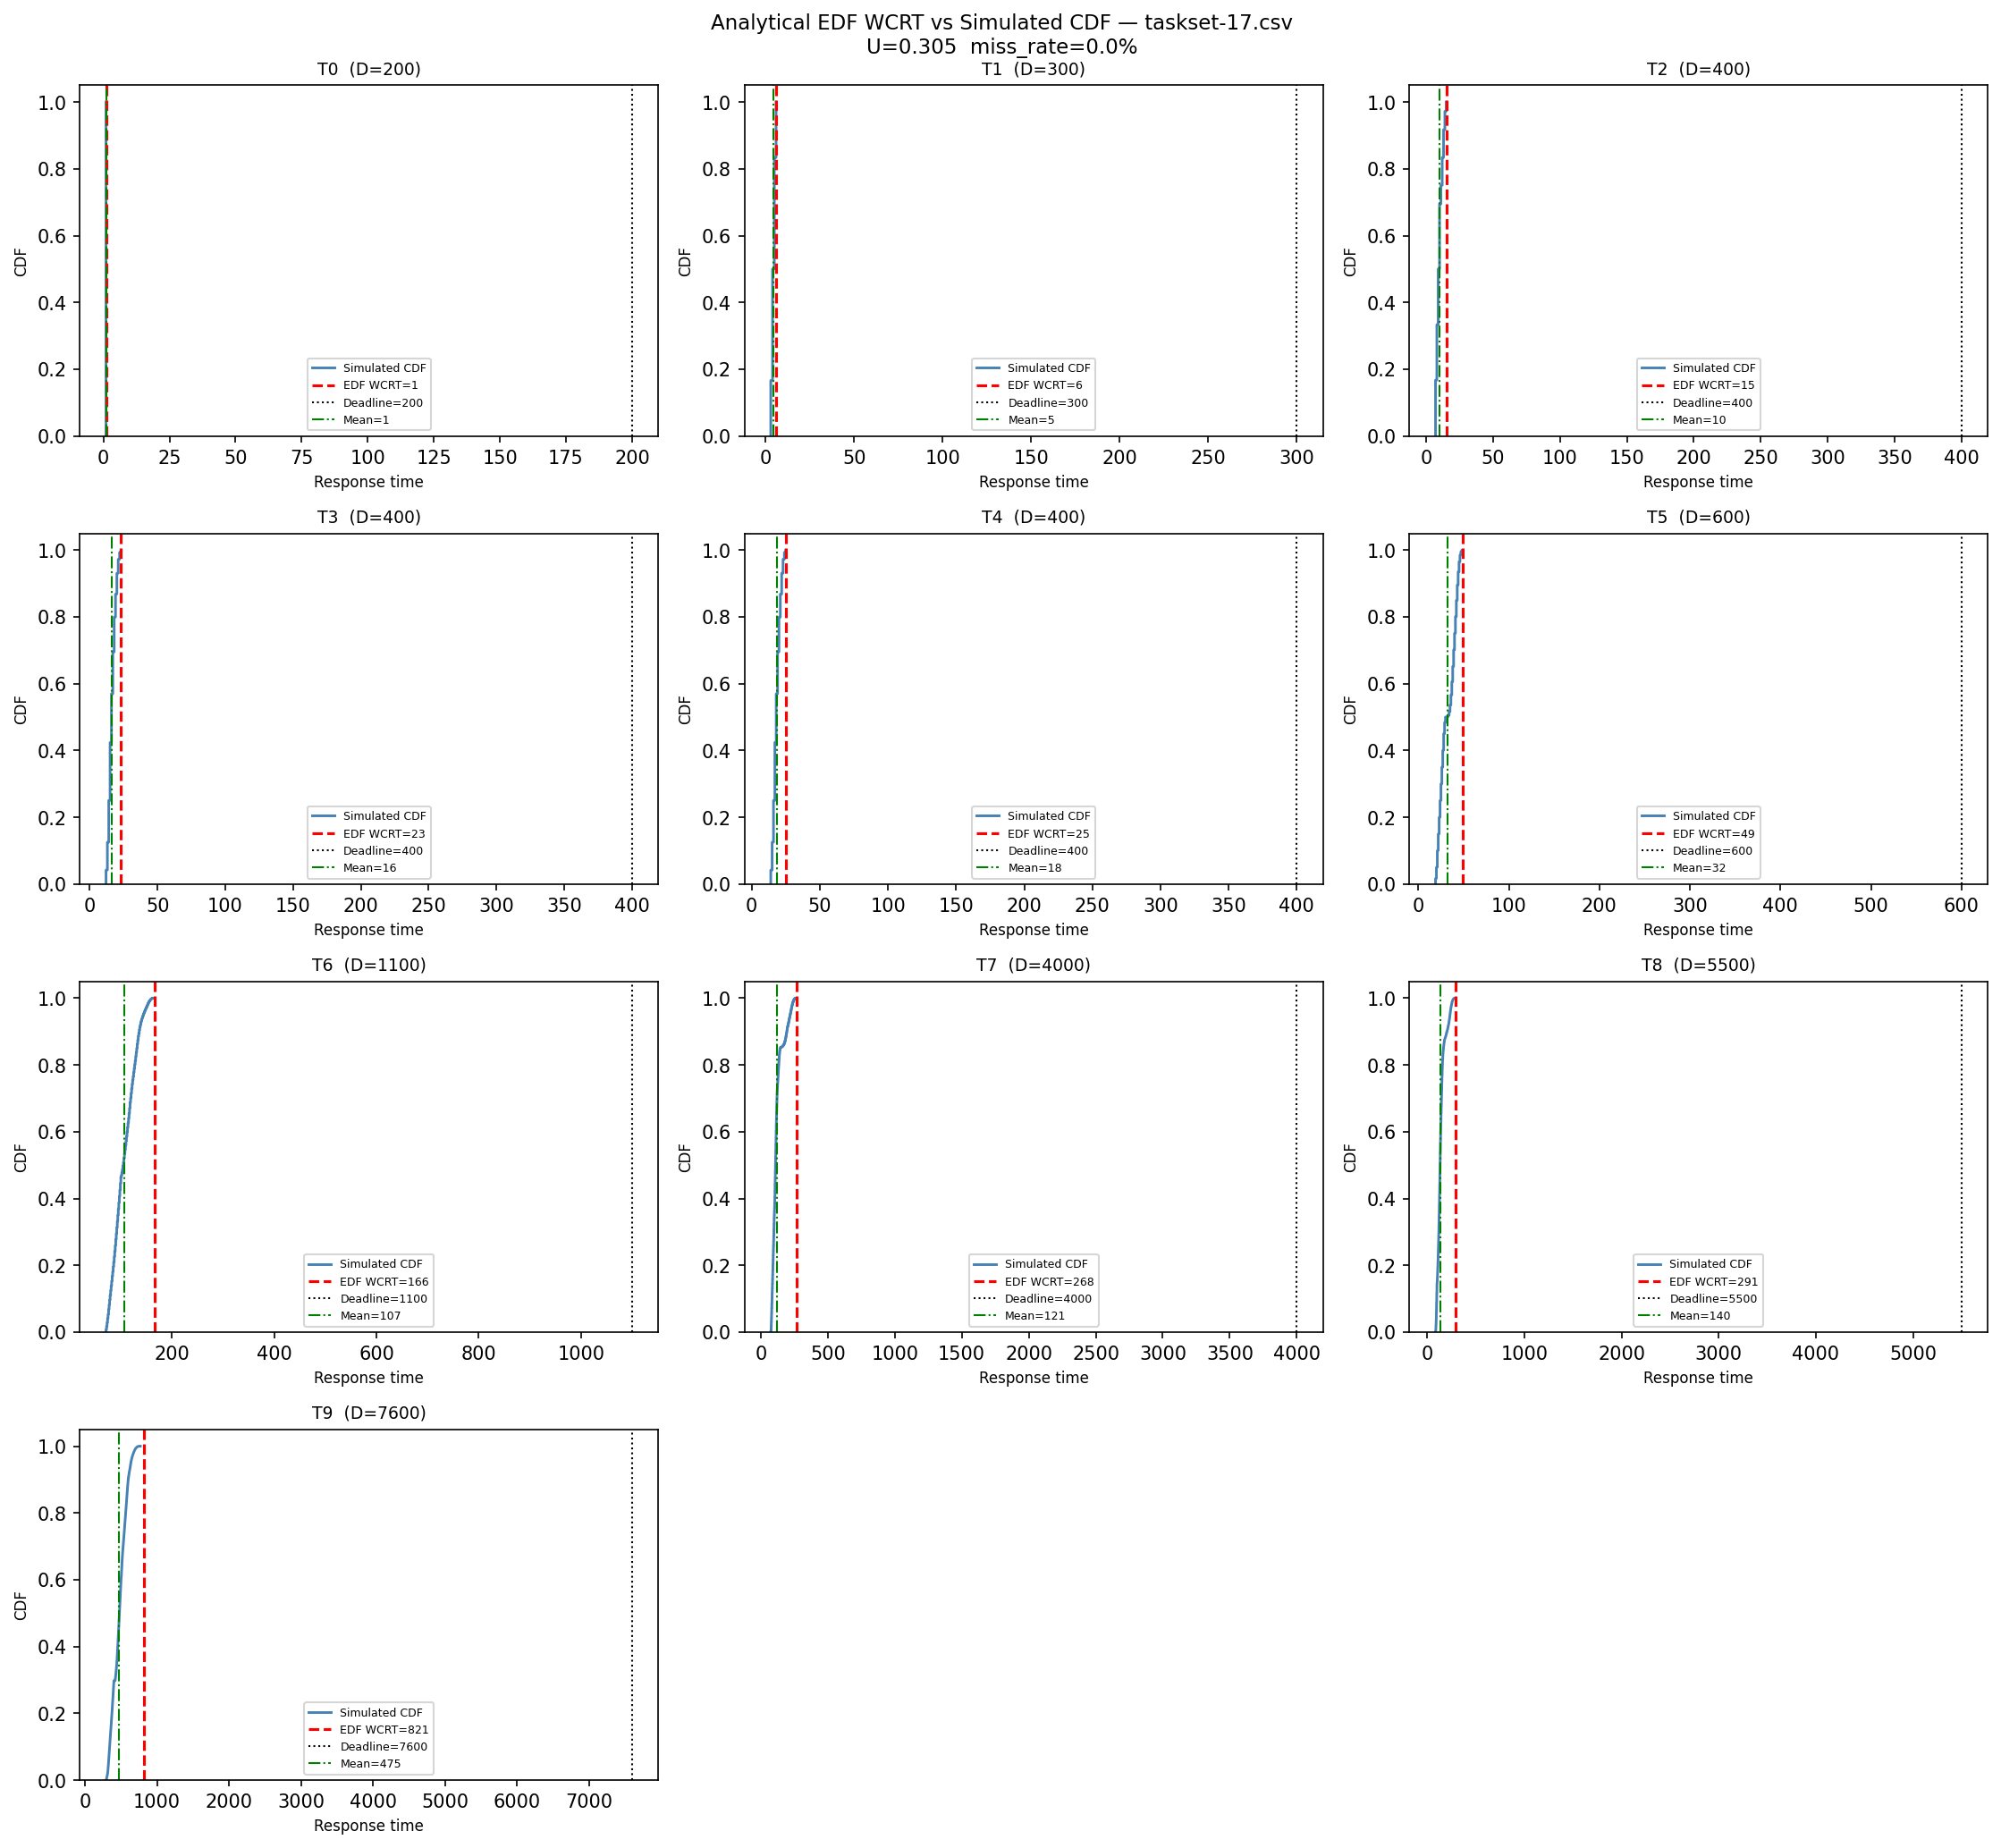
\includegraphics[width=\textwidth]{figures/cdf_u30_taskset-17.png}
    \caption{Simulated CDF vs.\ EDF WCRT at $U \approx 0.30$ (taskset-17).}
    \label{fig:cdf_u30}
\end{minipage}\hfill
\begin{minipage}{0.48\textwidth}
    \centering
    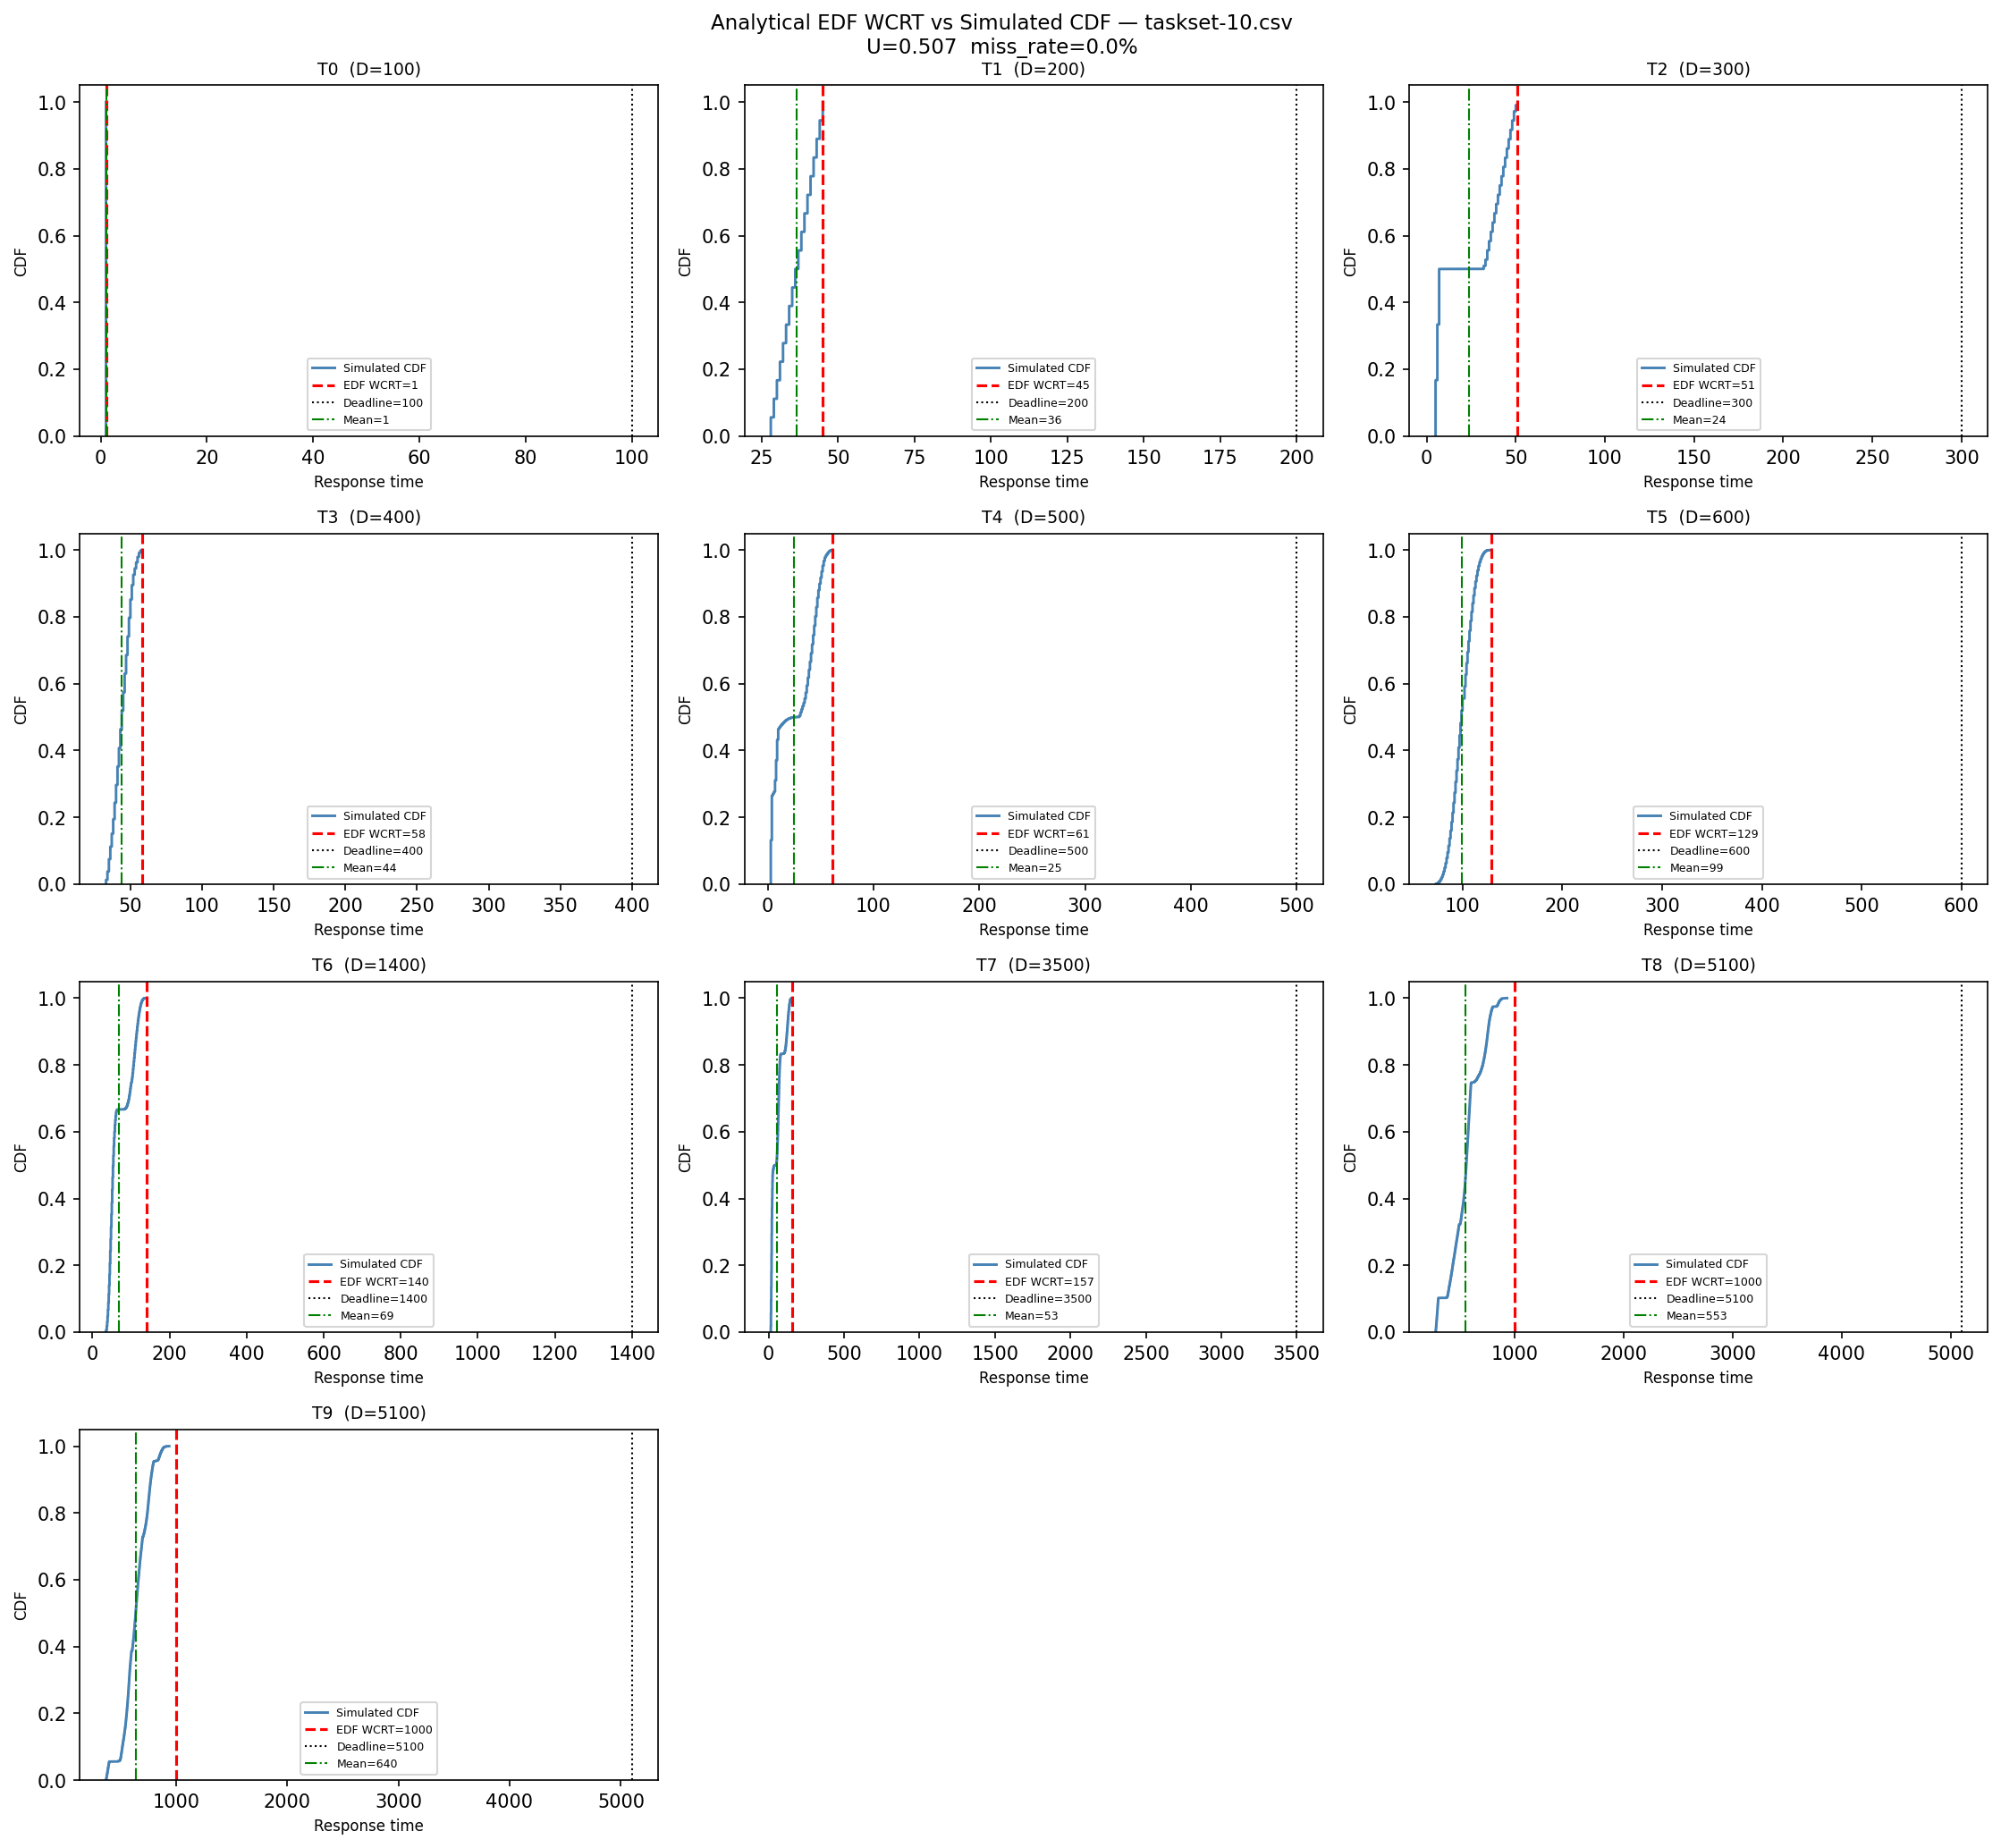
\includegraphics[width=\textwidth]{figures/cdf_u50_taskset-10.png}
    \caption{Simulated CDF vs.\ EDF WCRT at $U \approx 0.50$ (taskset-10).}
    \label{fig:cdf_u50}
\end{minipage}
\end{figure}

\begin{figure}[H]
\centering
\begin{minipage}{0.48\textwidth}
    \centering
    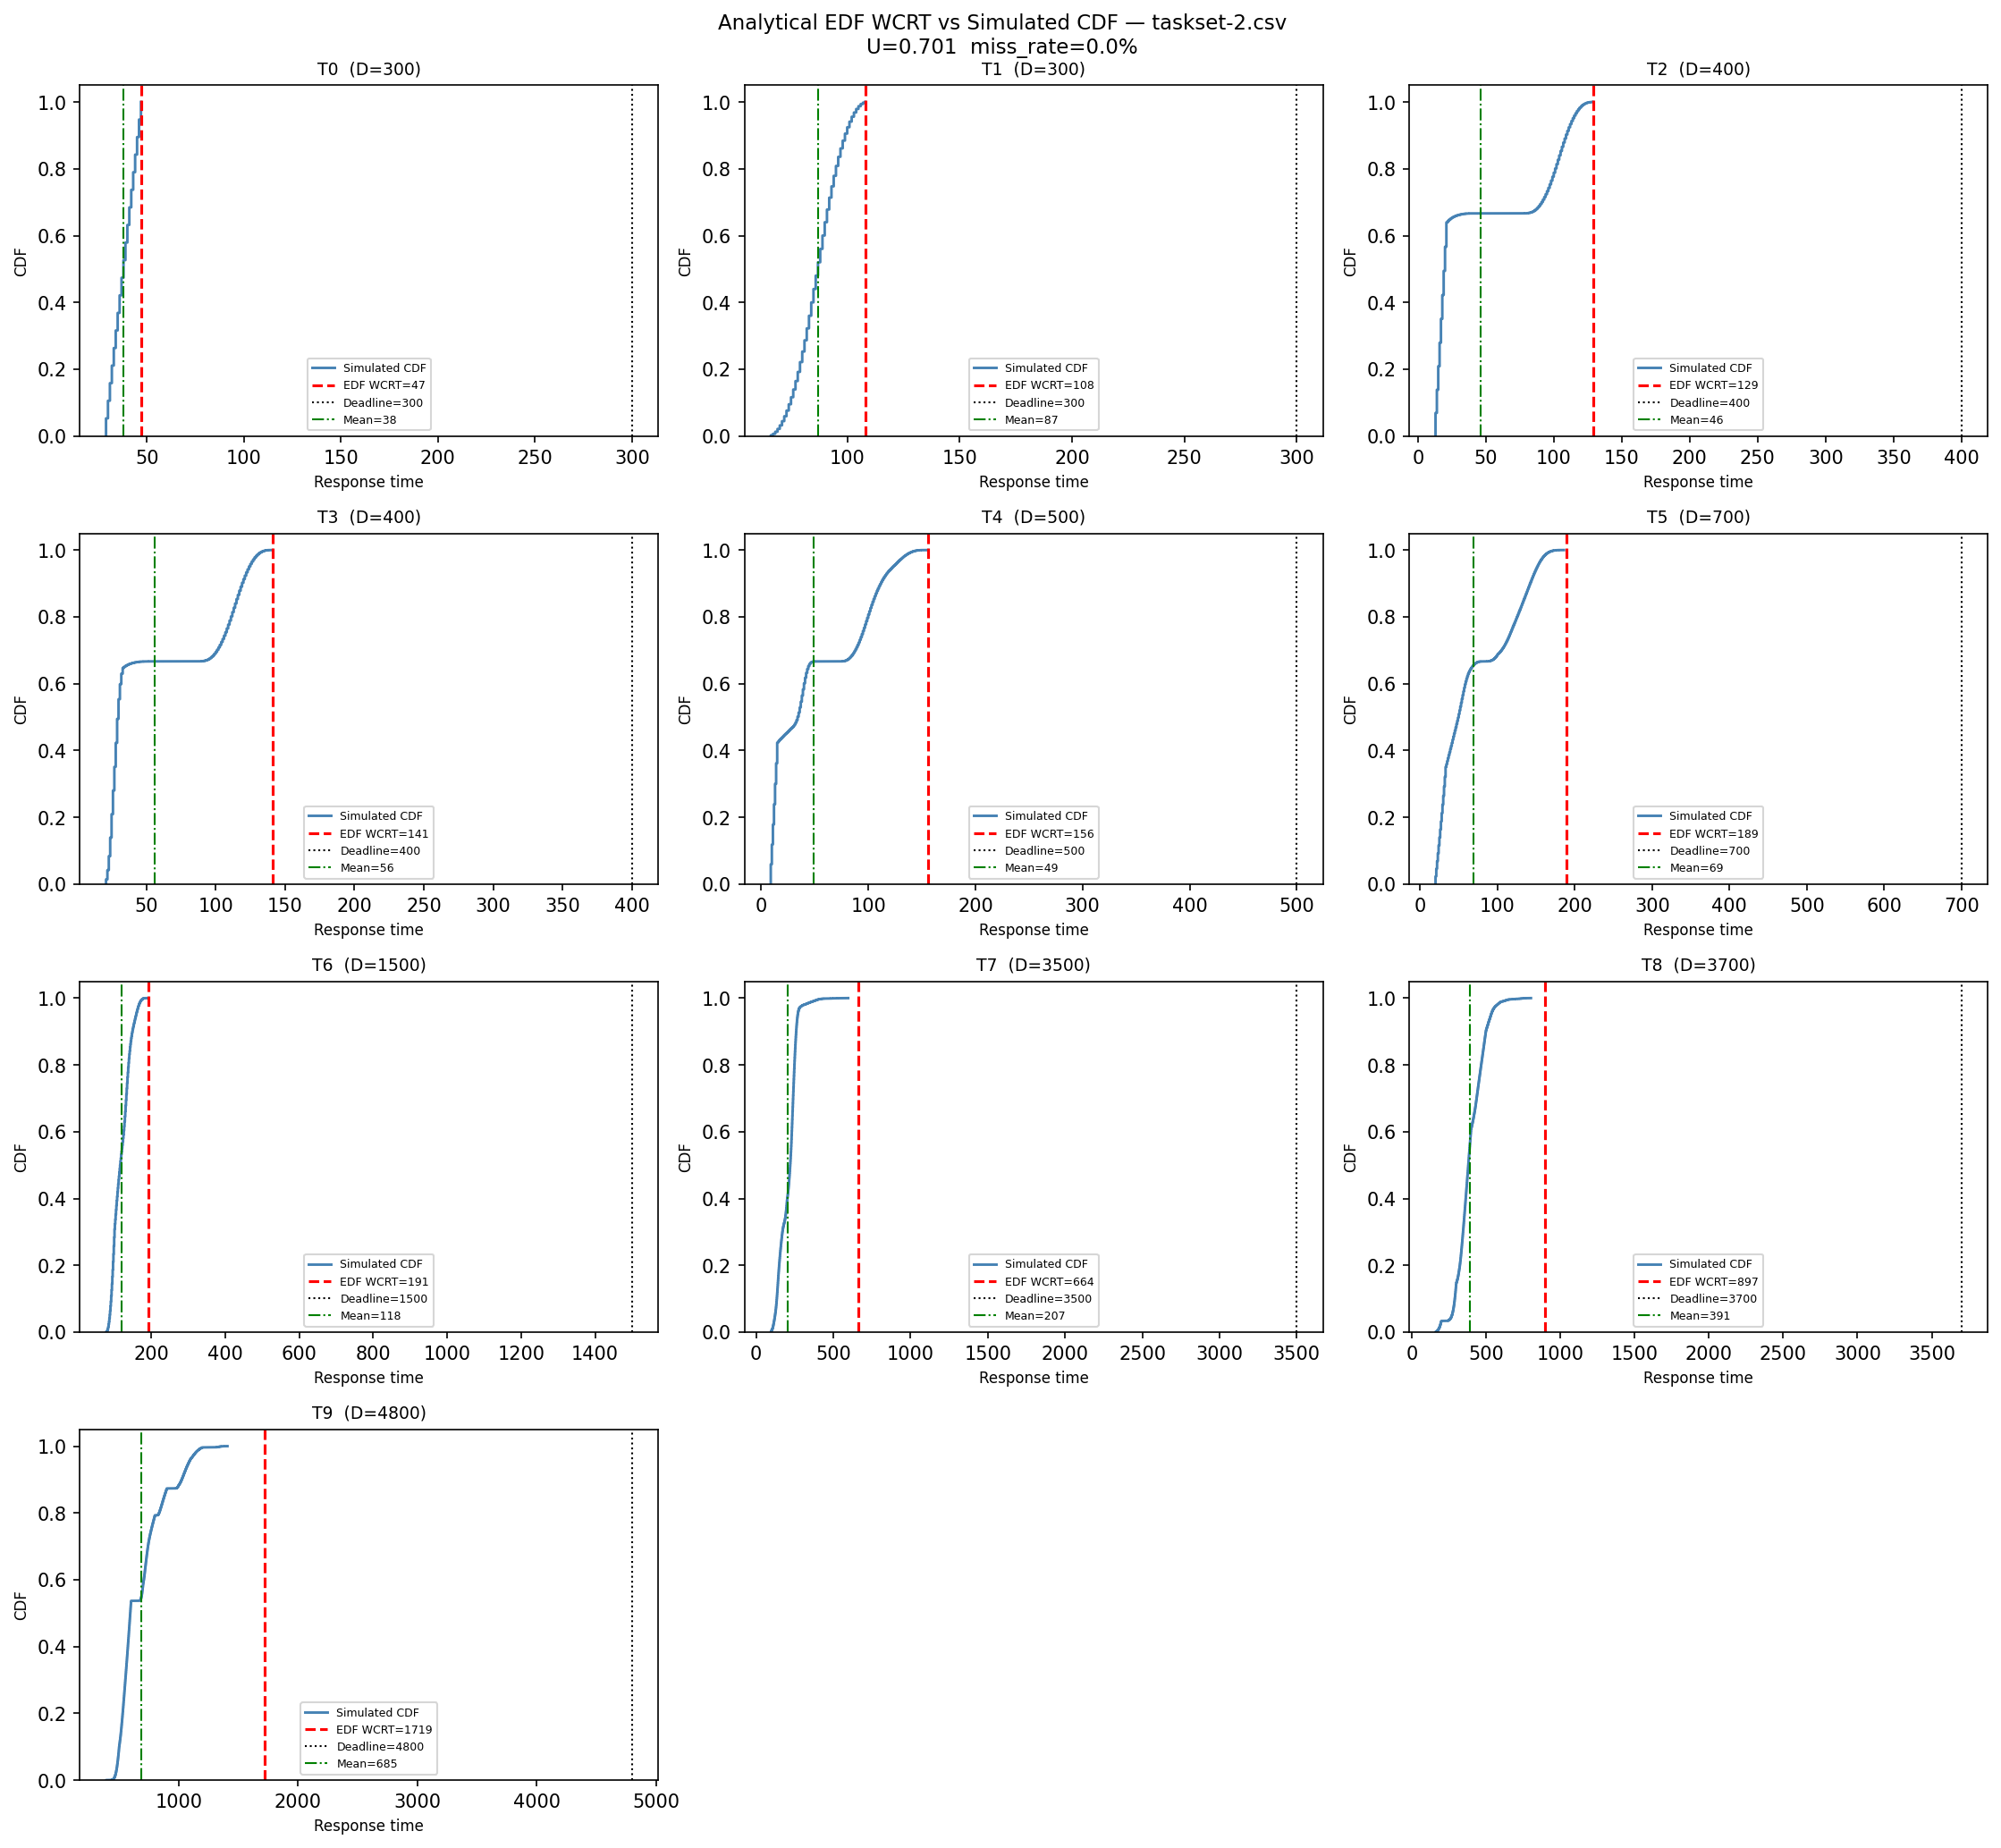
\includegraphics[width=\textwidth]{figures/cdf_u70_taskset-2.png}
    \caption{Simulated CDF vs.\ EDF WCRT at $U \approx 0.70$ (taskset-2).}
    \label{fig:cdf_u70}
\end{minipage}\hfill
\begin{minipage}{0.48\textwidth}
    \centering
    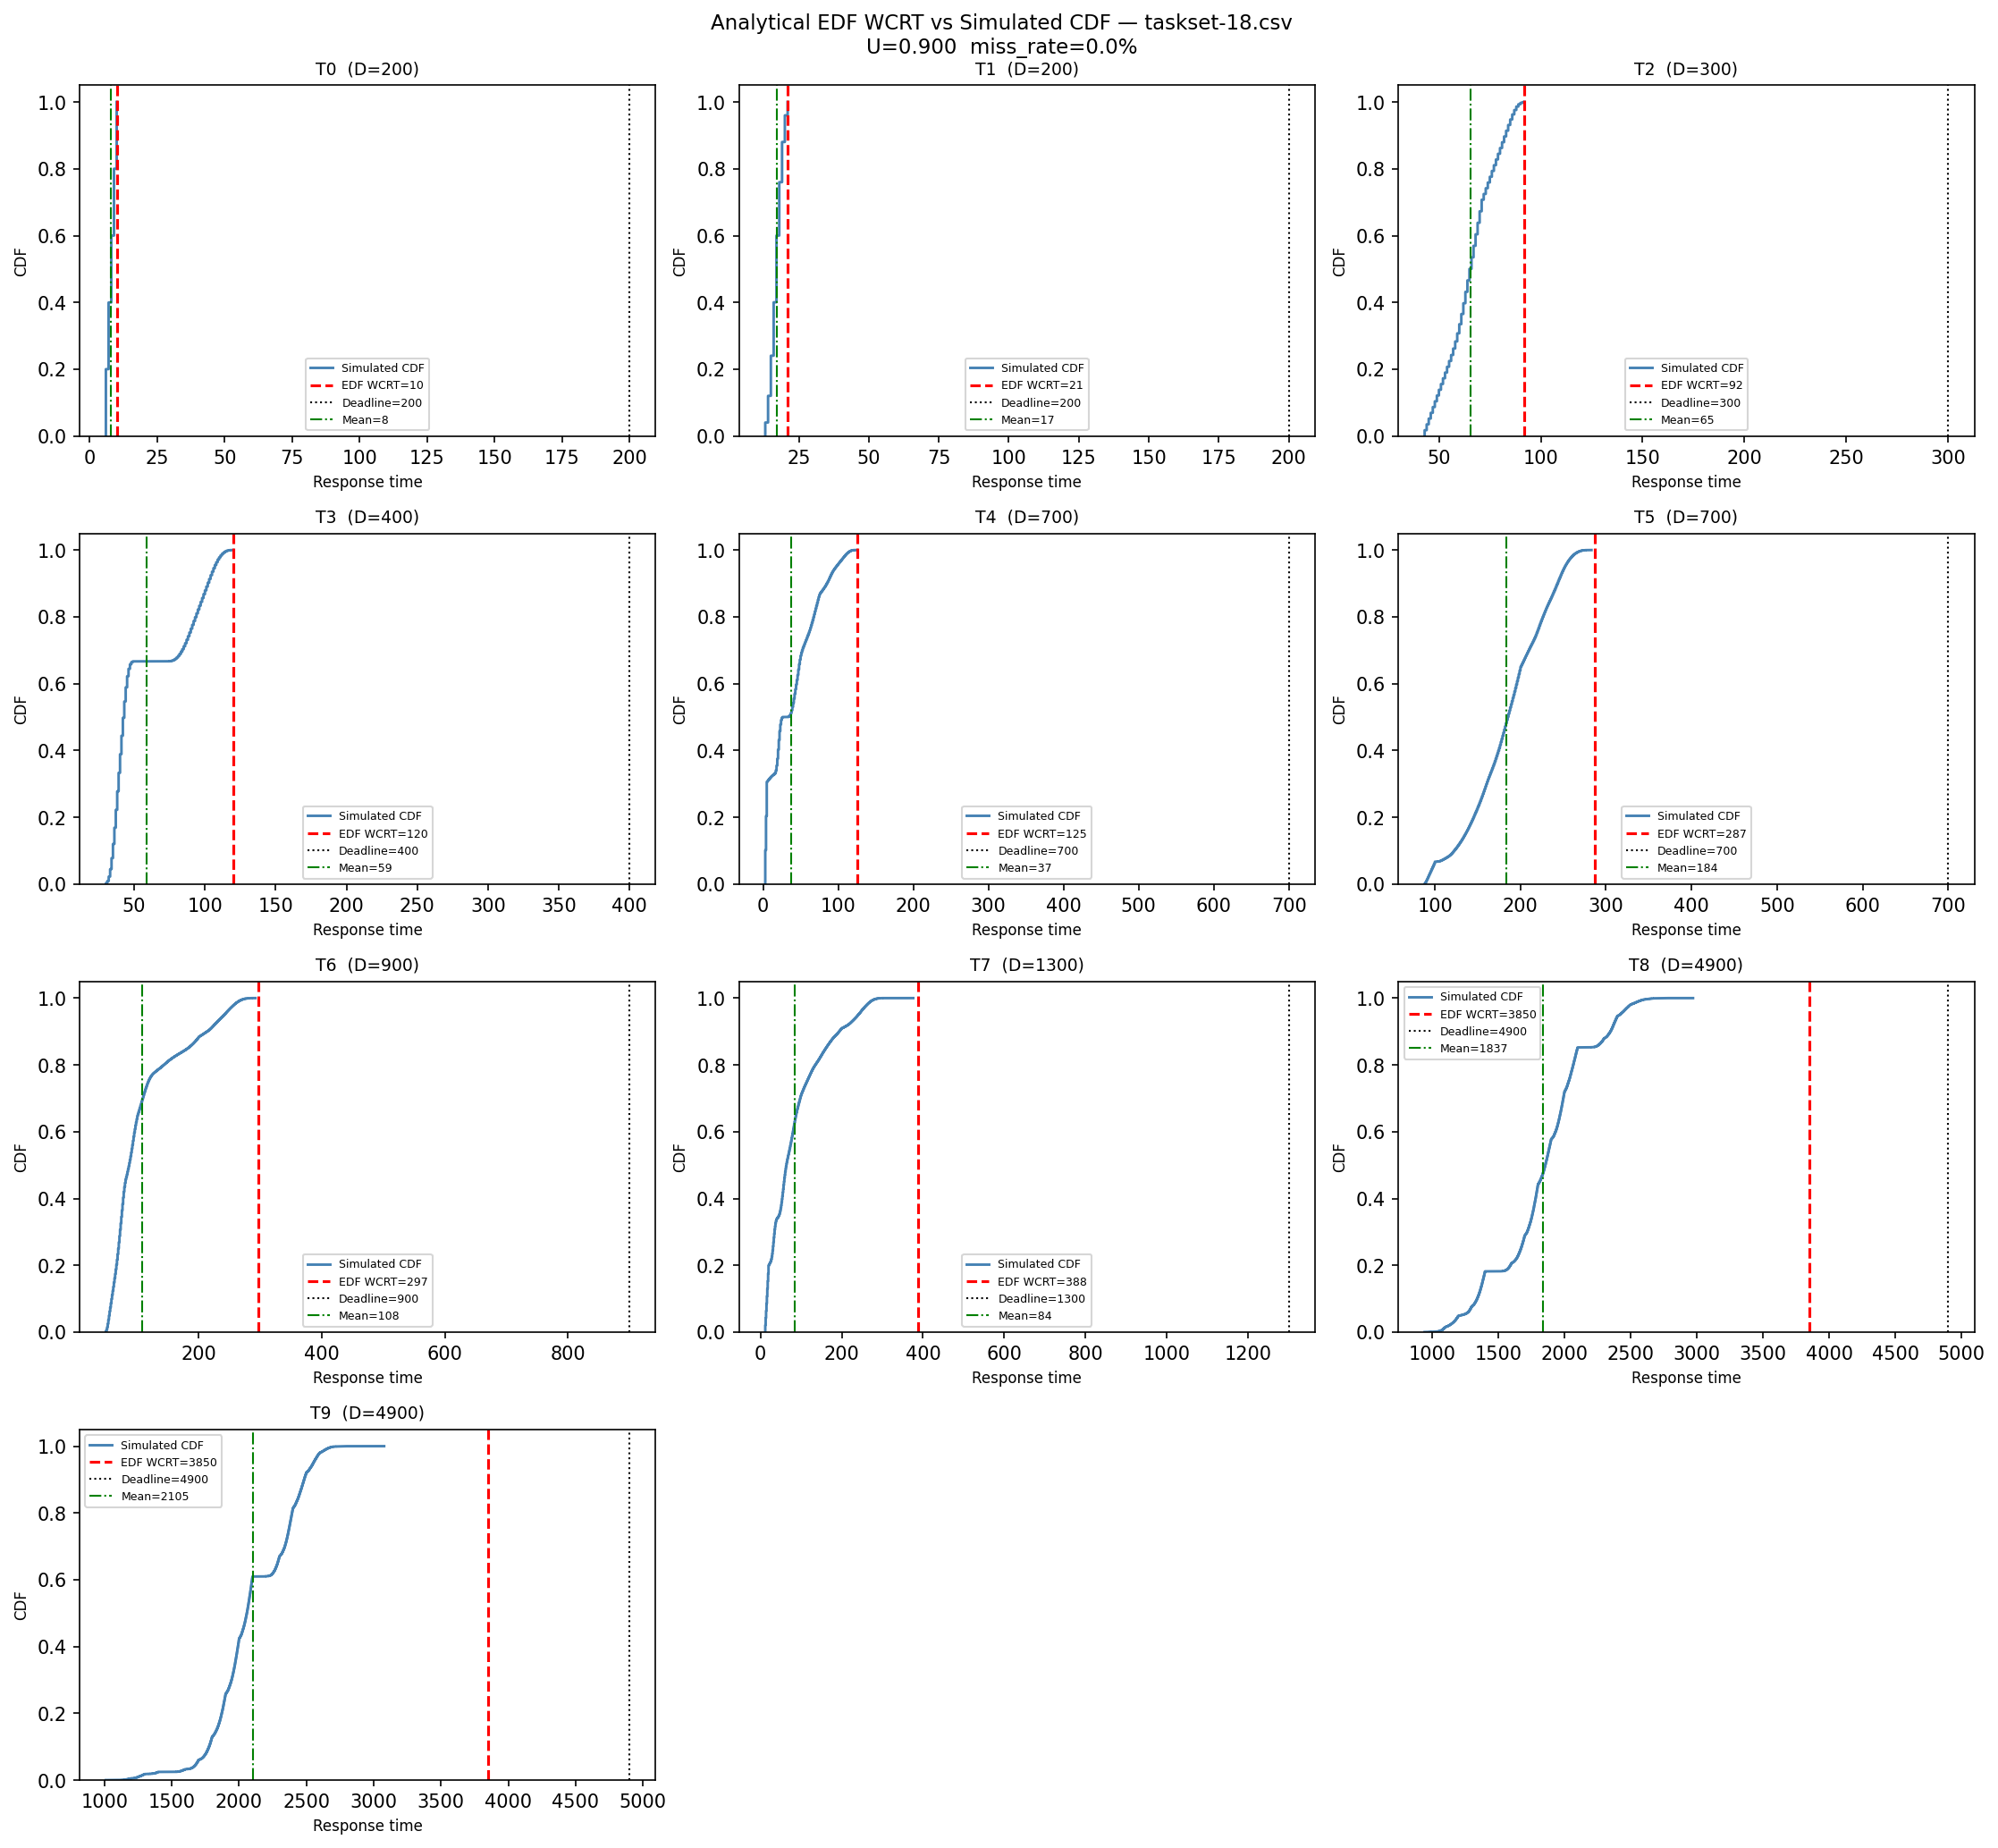
\includegraphics[width=\textwidth]{figures/cdf_u90_taskset-18.png}
    \caption{Simulated CDF vs.\ EDF WCRT at $U \approx 0.90$ (taskset-18).}
    \label{fig:cdf_u90}
\end{minipage}
\end{figure}

% ─────────────────────────────────────────────────────────────────────────────
\section{Extended Analysis: Harmonic Task Sets}
\label{sec:harmonic}
% ─────────────────────────────────────────────────────────────────────────────

\subsection{Schedulability Rates}

Table~\ref{tab:schedulability_harmonic} shows the schedulability results for the harmonic
benchmark. The overall picture is similar to the primary benchmark, with DM passing all sets
up to u70 and diverging from EDF only at u90. However, DM produces 4 failures at u90 (versus
2 in the non-harmonic benchmark), and EDF also fails 1 set at u90 (taskset-19, which has
$U > 1$ due to the harmonic period constraints). Overall, DM schedules 76/80 (95.0\%) and
EDF schedules 79/80 (98.8\%).

\begin{table}[H]
\centering
\caption{Schedulability results for harmonic task sets (20 sets each, $n=10$ tasks/set,
         300 sim.\ runs, seed = 42). All 80 sets are simulation-tractable.}
\label{tab:schedulability_harmonic}
\begin{tabular}{lrrrr}
\toprule
Level & Target $U$ & DM pass rate & EDF pass rate & Sets simulated \\
\midrule
u30   & 0.30 & 20/20 (100\%) & 20/20 (100\%) & 20/20 \\
u50   & 0.50 & 20/20 (100\%) & 20/20 (100\%) & 20/20 \\
u70   & 0.70 & 20/20 (100\%) & 20/20 (100\%) & 20/20 \\
u90   & 0.90 & 16/20~~(80\%) & 19/20~~(95\%) & 20/20 \\
\midrule
Total & --   & 76/80~~(95.0\%) & 79/80~~(98.8\%) & 80/80 (100\%) \\
\bottomrule
\end{tabular}
\end{table}

The most important result is in the final column: \emph{all 80 sets} are now fully simulated,
compared to only 14 in the non-harmonic benchmark. Figure~\ref{fig:sched_harmonic} compares
DM and EDF schedulability across utilisation levels.

\begin{figure}[H]
\centering
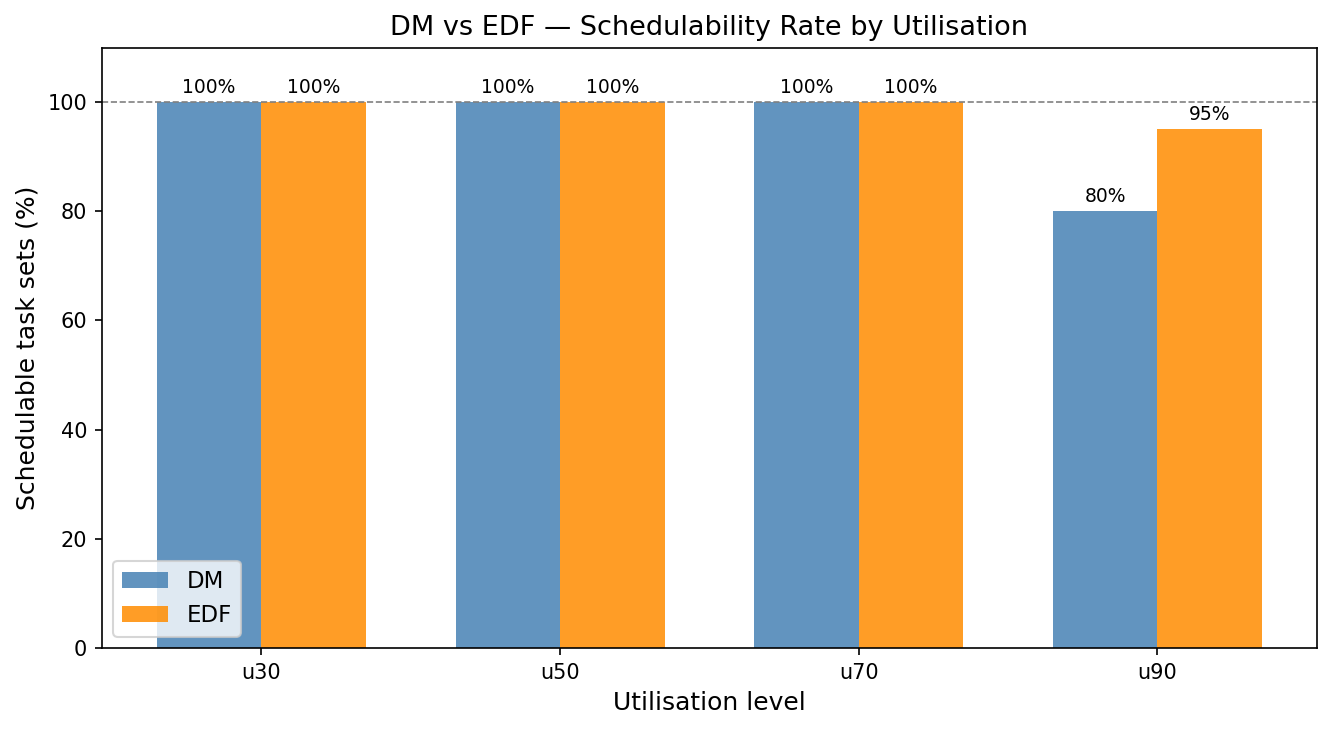
\includegraphics[width=0.72\textwidth]{figures/harmonic/schedulability_vs_utilization.png}
\caption{Schedulability rate (\%) for DM and EDF on the harmonic benchmark.
         DM drops to 80\% at $U \approx 0.90$; EDF drops to 95\% due to one
         over-utilised set (taskset-19, $U > 1$).}
\label{fig:sched_harmonic}
\end{figure}

\subsection{WCRT Comparison}

Figures~\ref{fig:wcrt_h_u30}--\ref{fig:wcrt_h_u90} show per-task WCRTs under DM and EDF
for one representative harmonic set at each utilisation level. The same qualitative pattern
holds as in the non-harmonic results: DM WCRTs rise steeply for lower-priority tasks due to
accumulated interference, while EDF distributes response times more evenly. The WCRTs are
generally comparable in magnitude to the non-harmonic sets at the same utilisation level,
confirming that the harmonic period structure affects tractability but not the fundamental
scheduling behaviour.

\begin{figure}[H]
\centering
\begin{minipage}{0.48\textwidth}
    \centering
    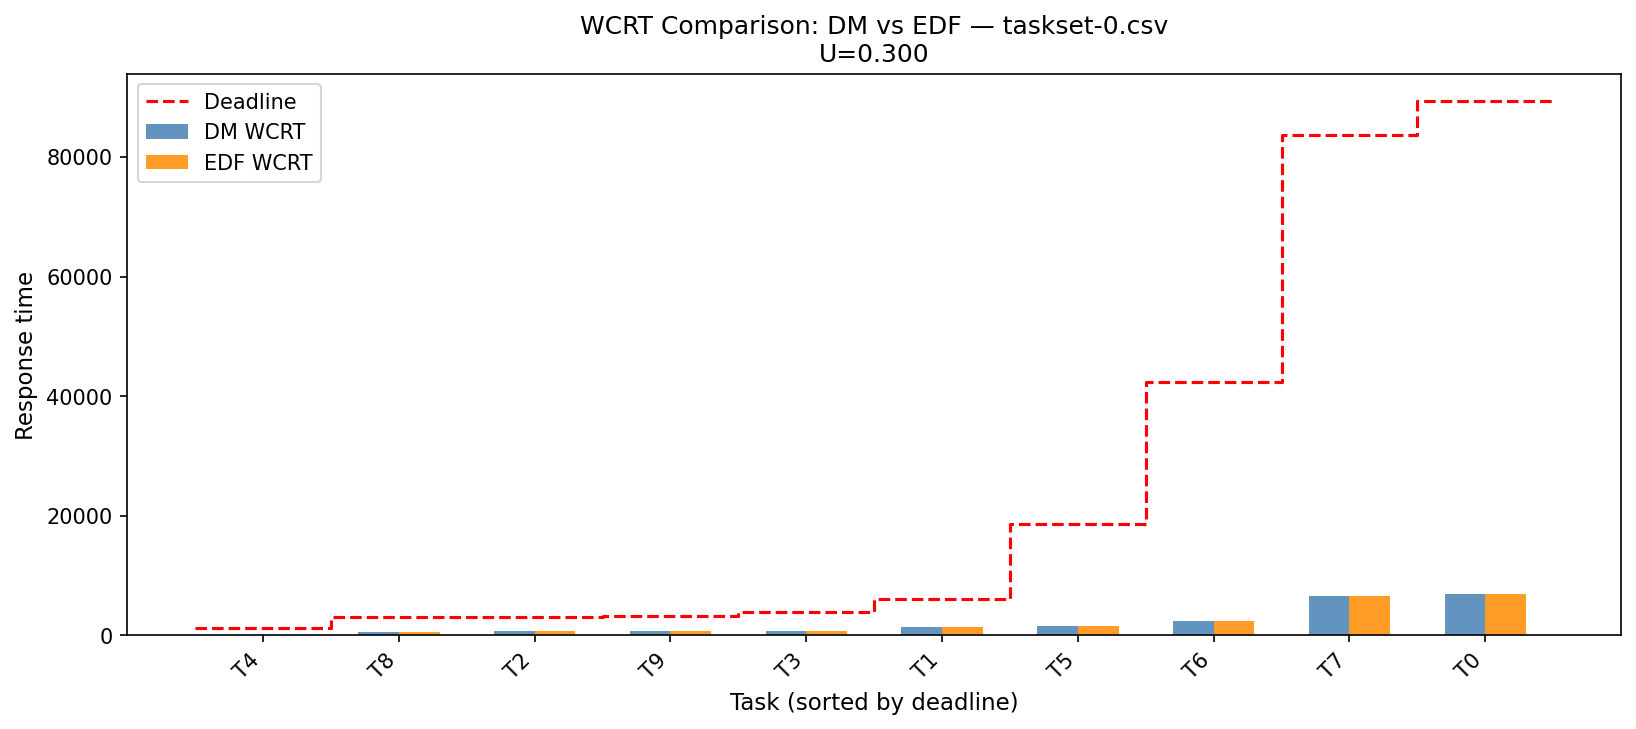
\includegraphics[width=\textwidth]{figures/harmonic/wcrt_u30_taskset-0.png}
    \caption{WCRT: DM vs.\ EDF at $U \approx 0.30$, harmonic (taskset-0).}
    \label{fig:wcrt_h_u30}
\end{minipage}\hfill
\begin{minipage}{0.48\textwidth}
    \centering
    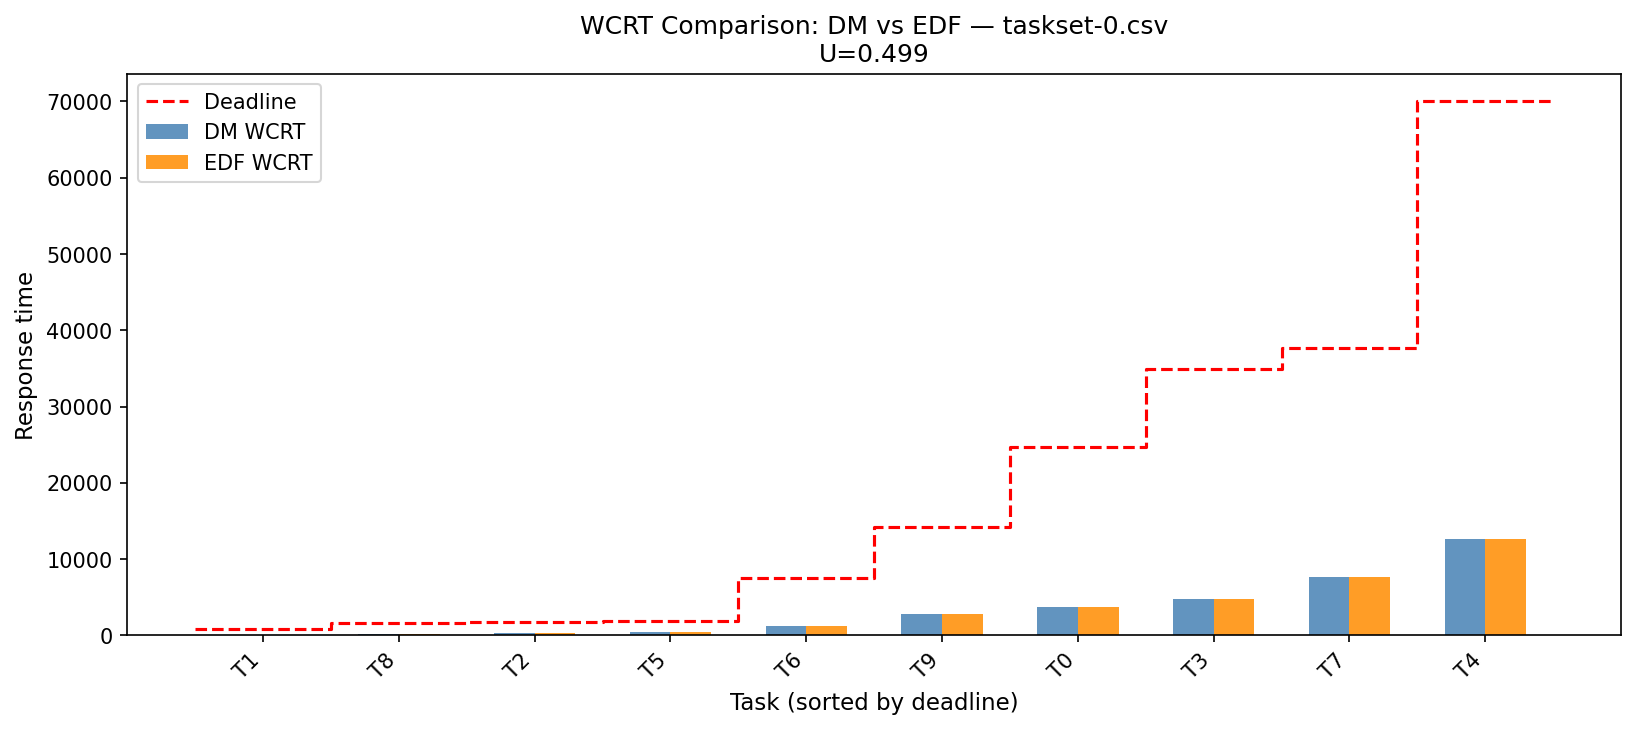
\includegraphics[width=\textwidth]{figures/harmonic/wcrt_u50_taskset-0.png}
    \caption{WCRT: DM vs.\ EDF at $U \approx 0.50$, harmonic (taskset-0).}
    \label{fig:wcrt_h_u50}
\end{minipage}
\end{figure}

\begin{figure}[H]
\centering
\begin{minipage}{0.48\textwidth}
    \centering
    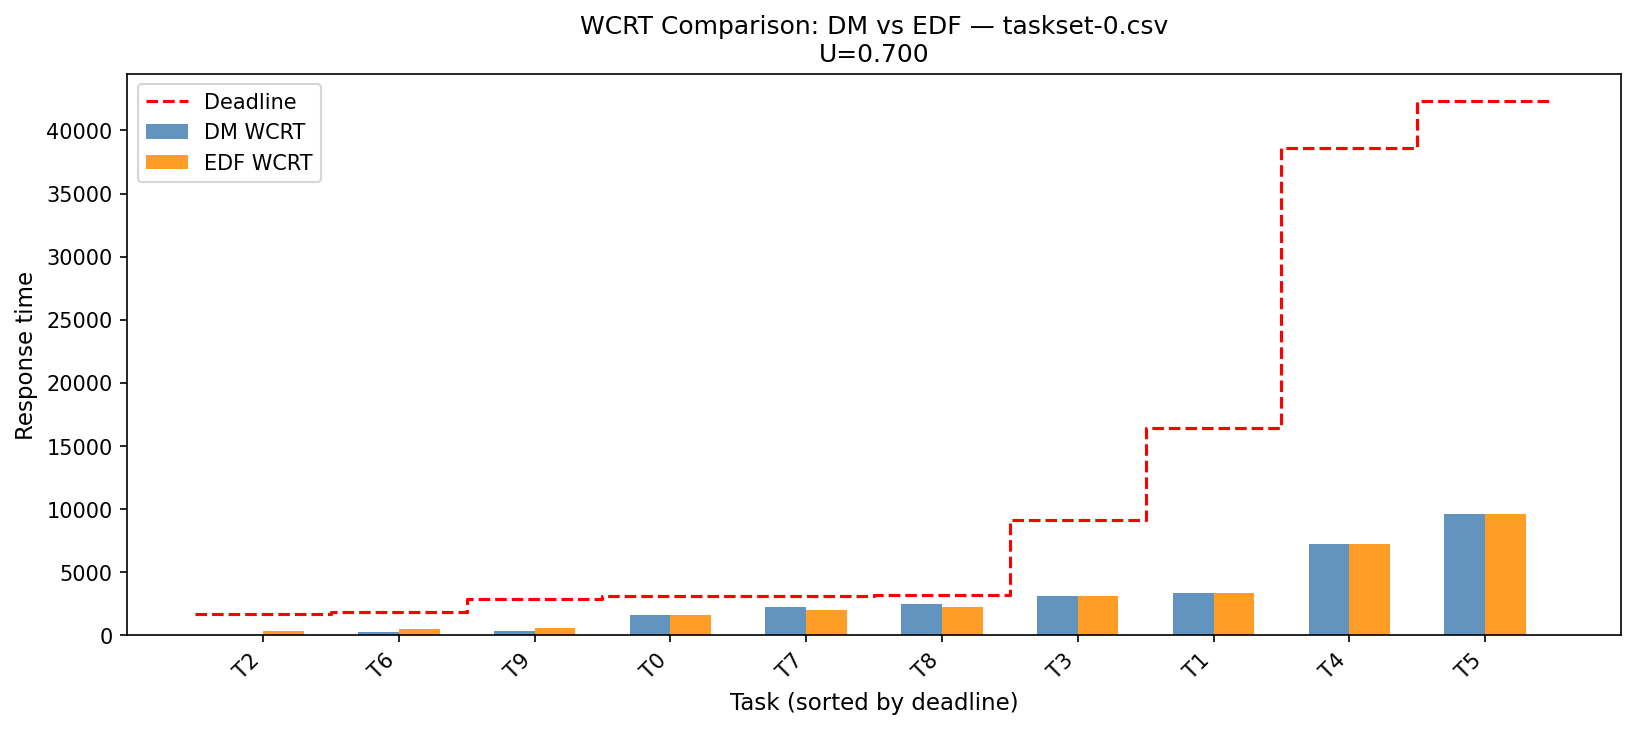
\includegraphics[width=\textwidth]{figures/harmonic/wcrt_u70_taskset-0.png}
    \caption{WCRT: DM vs.\ EDF at $U \approx 0.70$, harmonic (taskset-0).}
    \label{fig:wcrt_h_u70}
\end{minipage}\hfill
\begin{minipage}{0.48\textwidth}
    \centering
    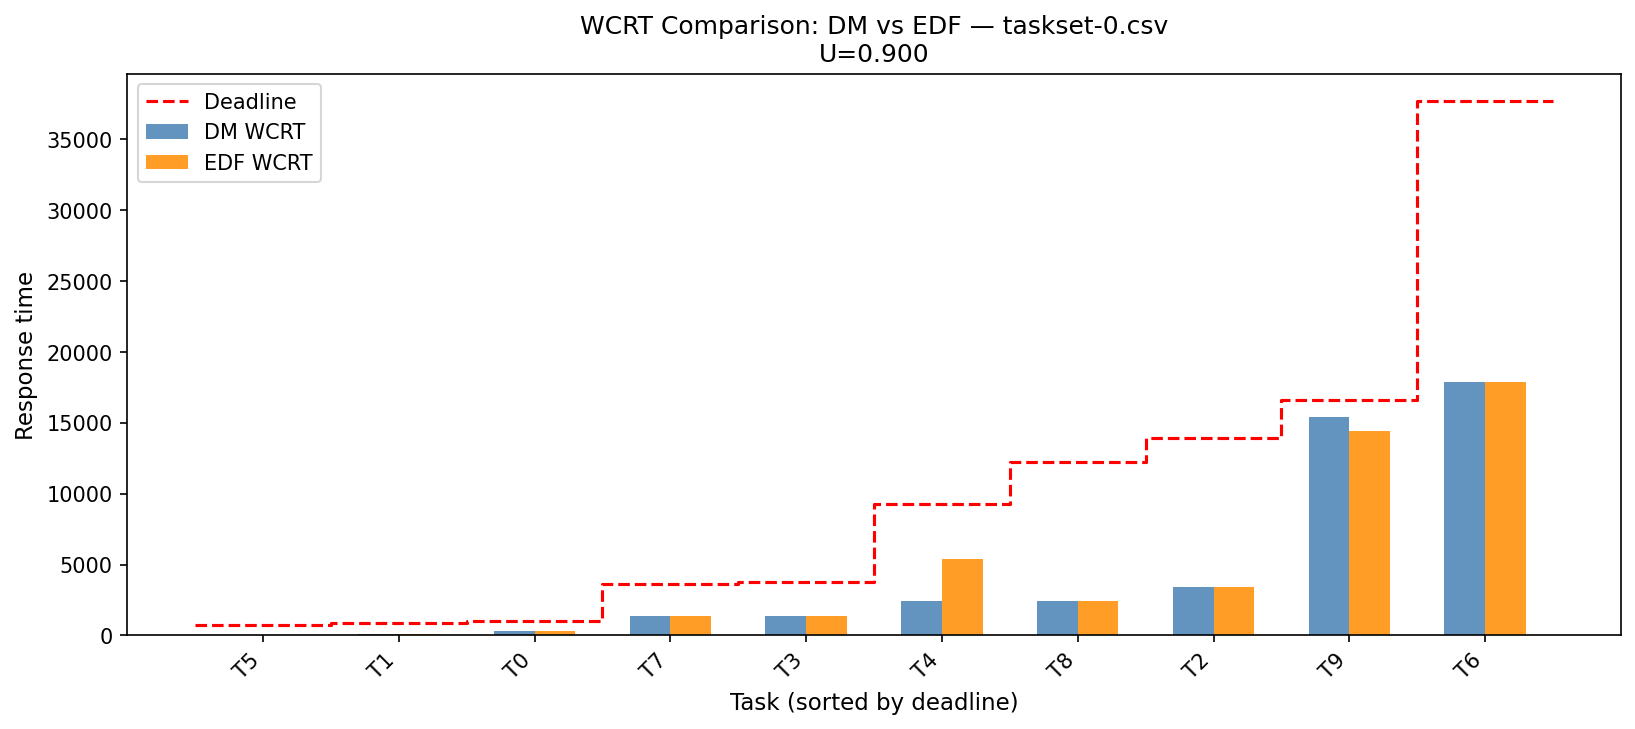
\includegraphics[width=\textwidth]{figures/harmonic/wcrt_u90_taskset-0.png}
    \caption{WCRT: DM vs.\ EDF at $U \approx 0.90$, harmonic (taskset-0, DM passes).}
    \label{fig:wcrt_h_u90}
\end{minipage}
\end{figure}

\subsection{Analytical Bounds versus Simulated Response Times}

With all 80 sets now tractable, the Monte Carlo validation is complete across the full
benchmark for the first time. Zero deadline misses were observed in every set and every
run. Figures~\ref{fig:cdf_h_u30}--\ref{fig:cdf_h_u90} show the empirical CDFs for one
representative set per utilisation level. The same conclusions hold as in
Section~\ref{sec:results}: the analytical EDF WCRT is a valid but pessimistic bound, with
mean observed response times at roughly 30--60\% of the WCRT and P95/P99 clustering near
the mean. The harmonic results therefore extend this finding from 14 sets to all 80,
substantially strengthening the empirical validation.

\begin{figure}[H]
\centering
\begin{minipage}{0.48\textwidth}
    \centering
    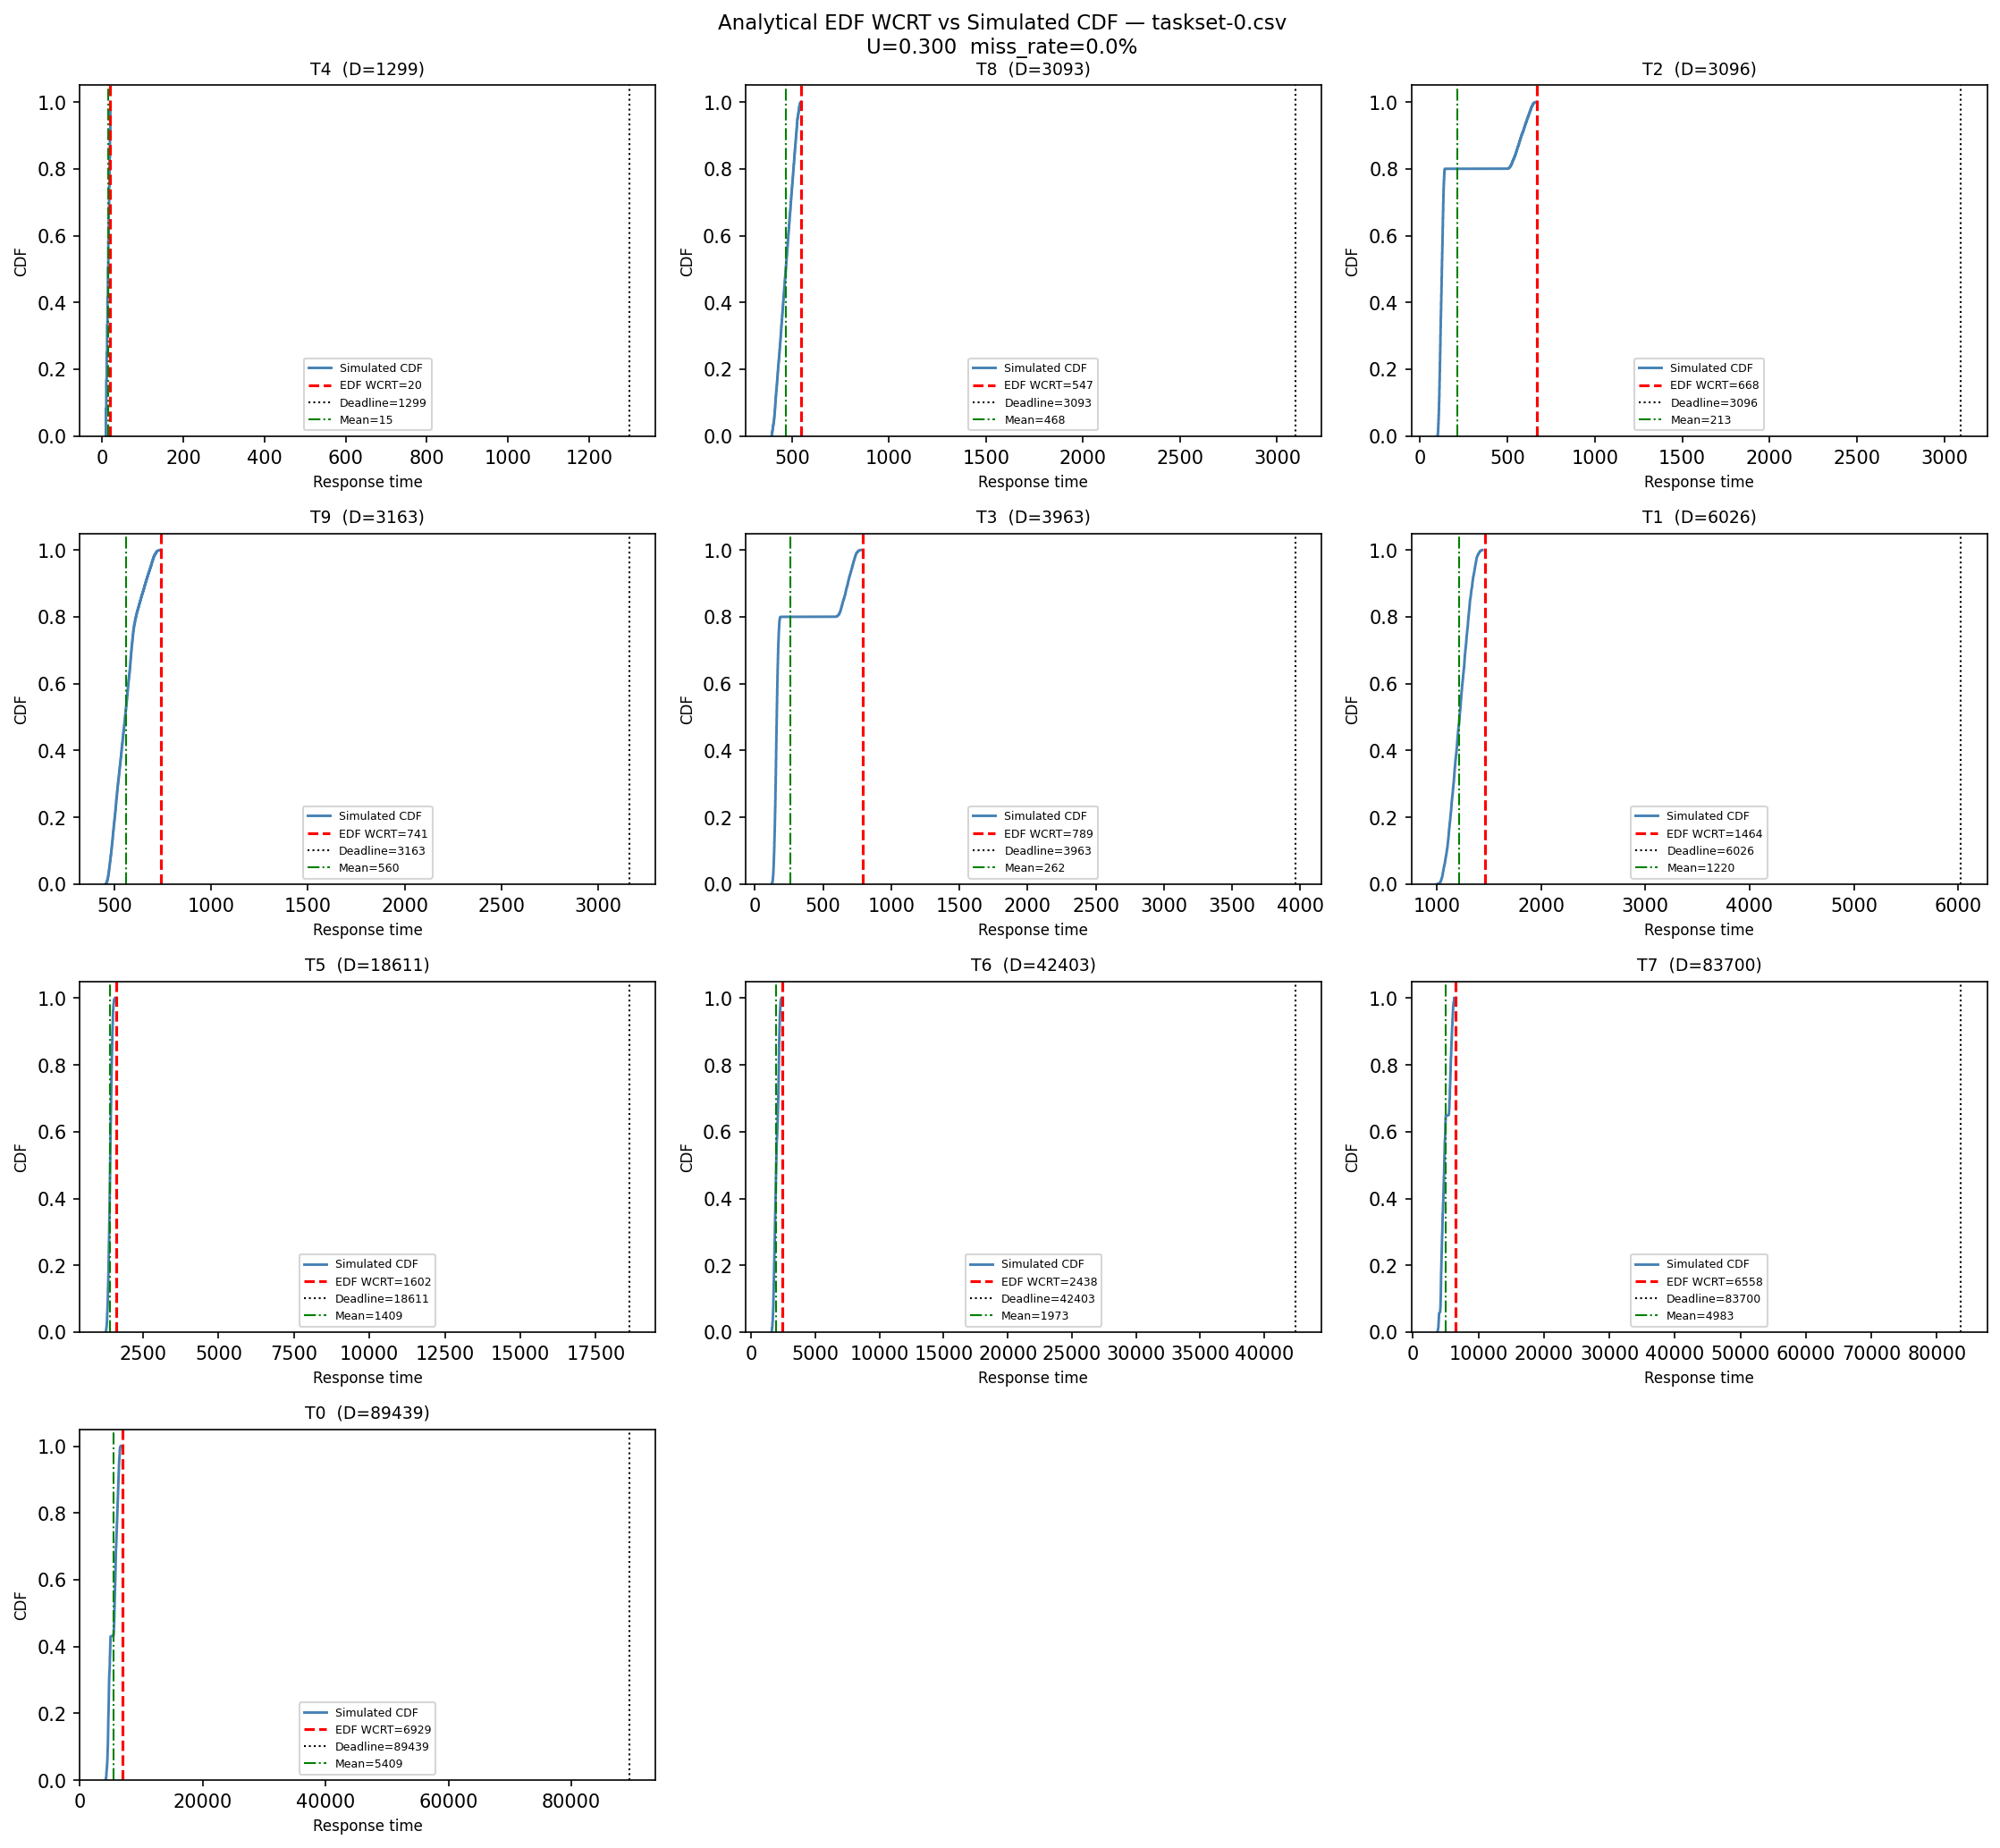
\includegraphics[width=\textwidth]{figures/harmonic/cdf_u30_taskset-0.png}
    \caption{Simulated CDF vs.\ EDF WCRT at $U \approx 0.30$, harmonic (taskset-0).}
    \label{fig:cdf_h_u30}
\end{minipage}\hfill
\begin{minipage}{0.48\textwidth}
    \centering
    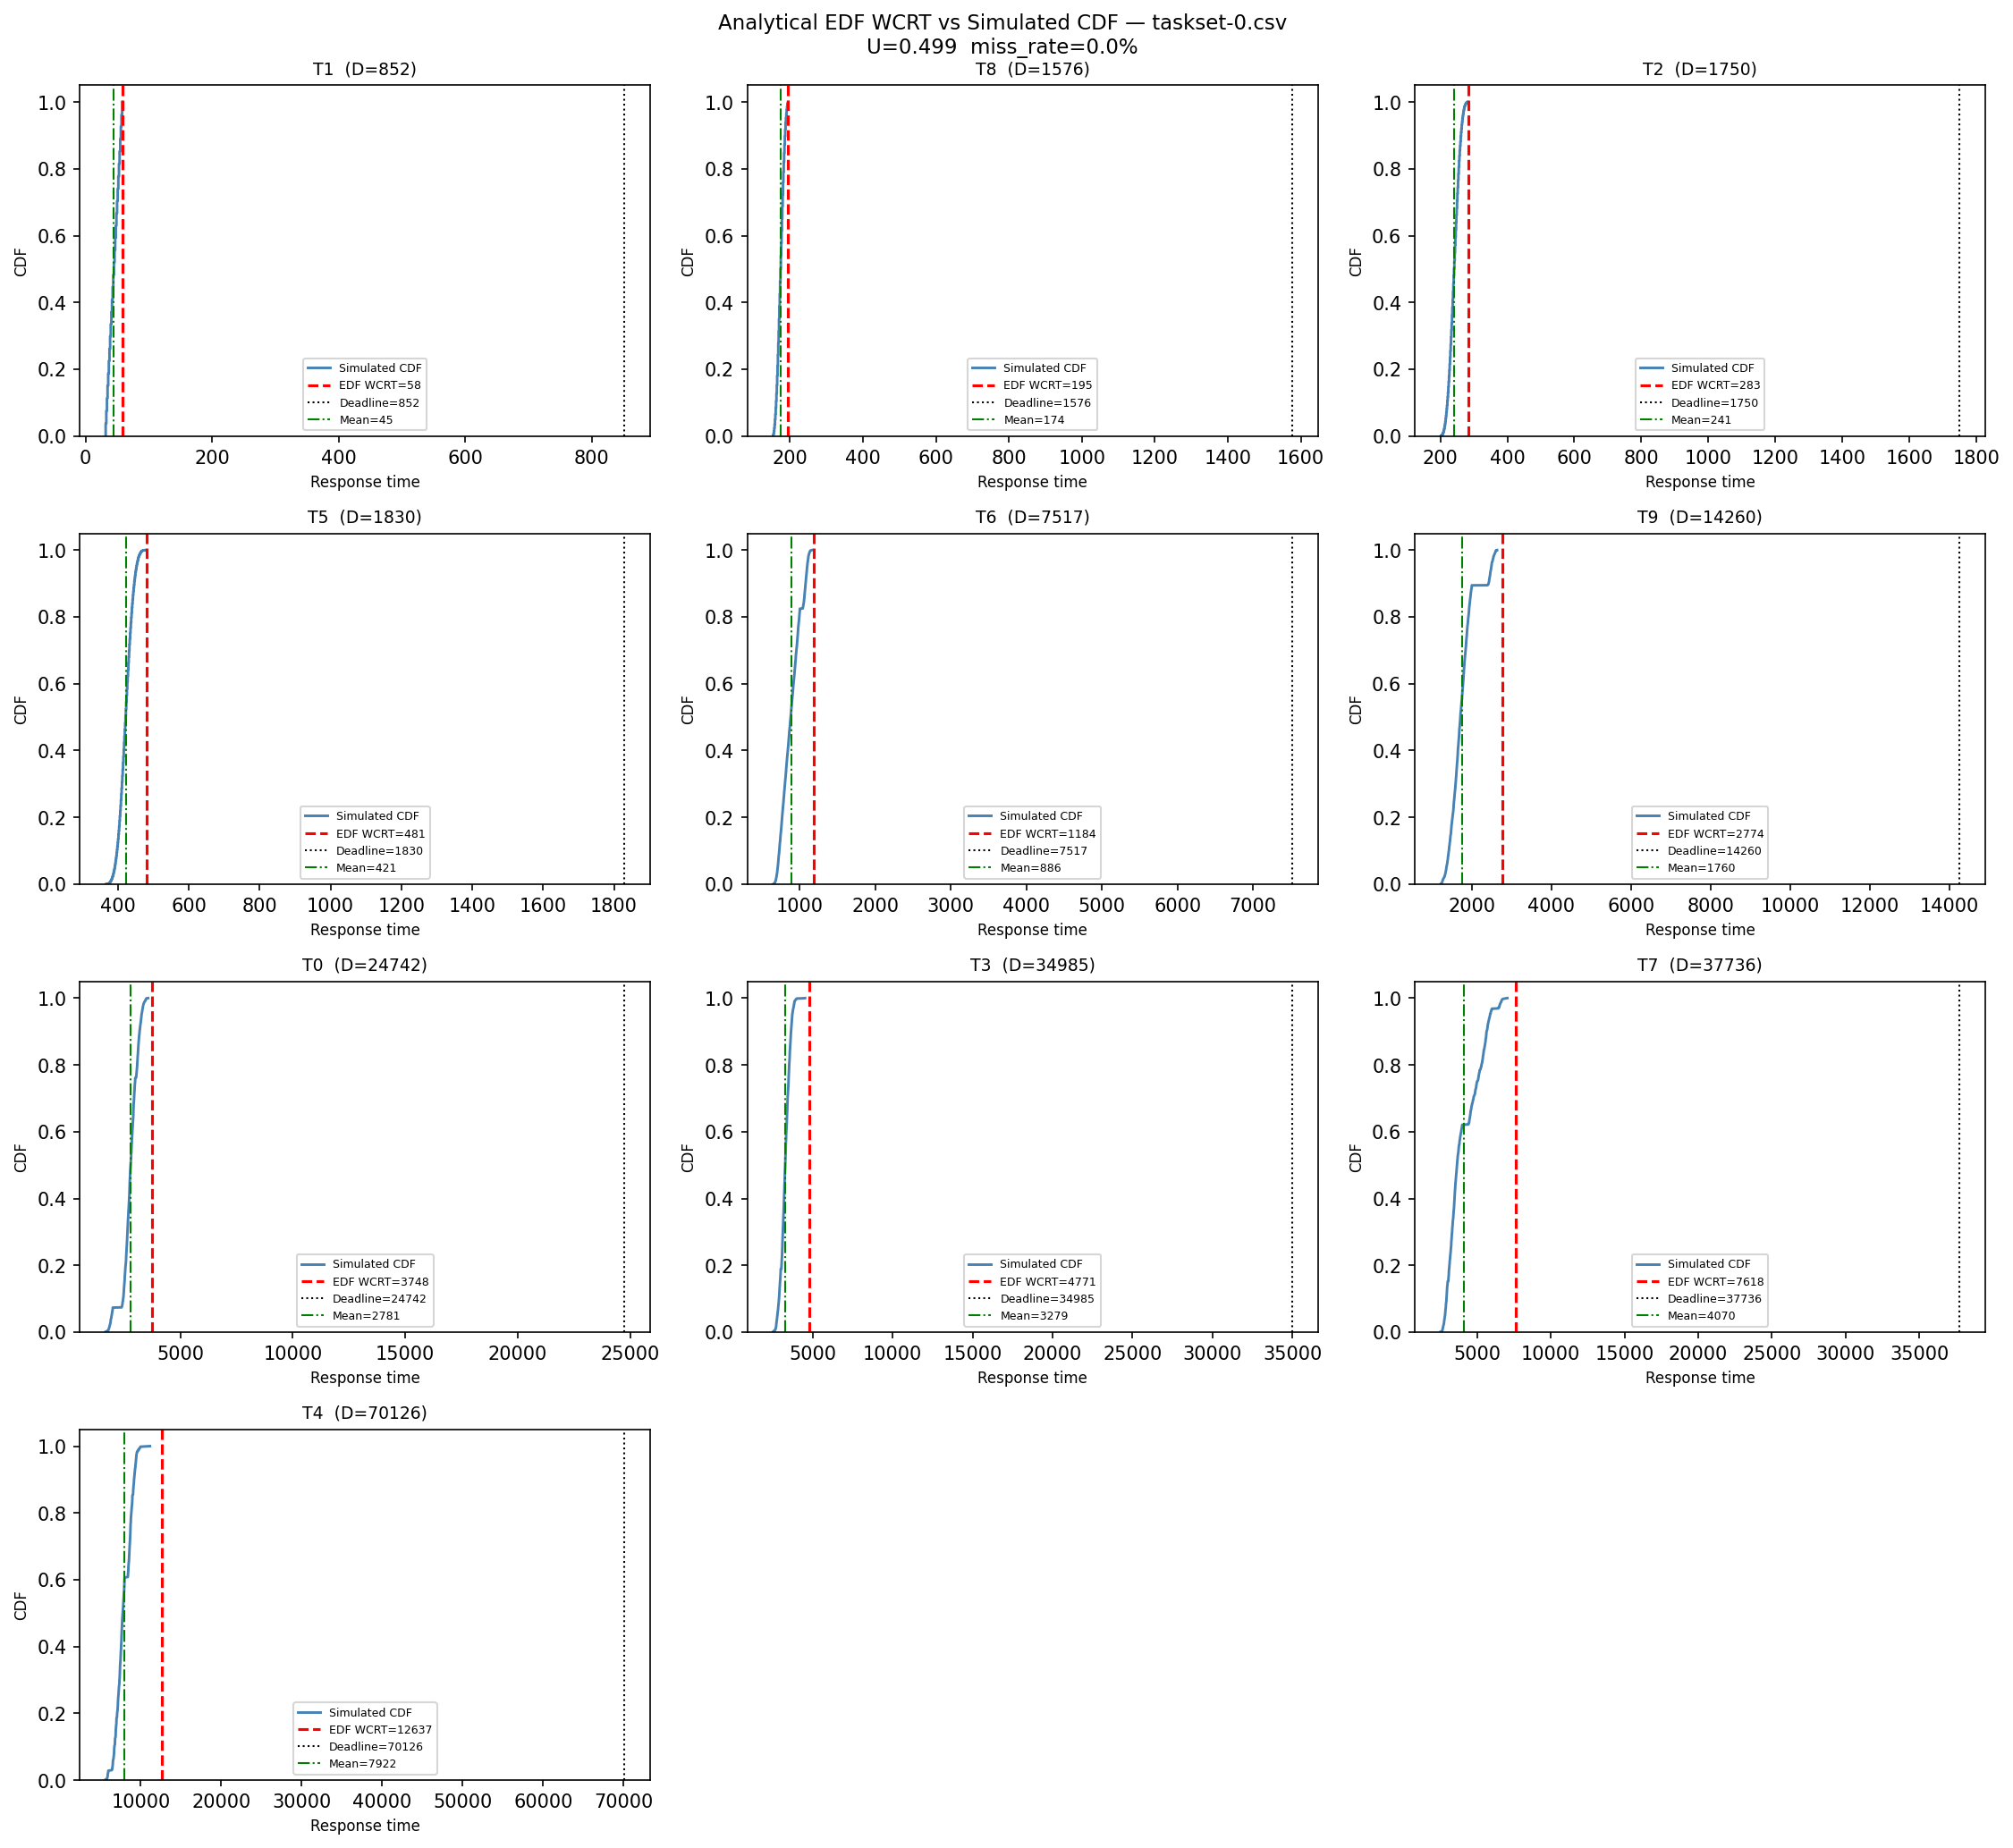
\includegraphics[width=\textwidth]{figures/harmonic/cdf_u50_taskset-0.png}
    \caption{Simulated CDF vs.\ EDF WCRT at $U \approx 0.50$, harmonic (taskset-0).}
    \label{fig:cdf_h_u50}
\end{minipage}
\end{figure}

\begin{figure}[H]
\centering
\begin{minipage}{0.48\textwidth}
    \centering
    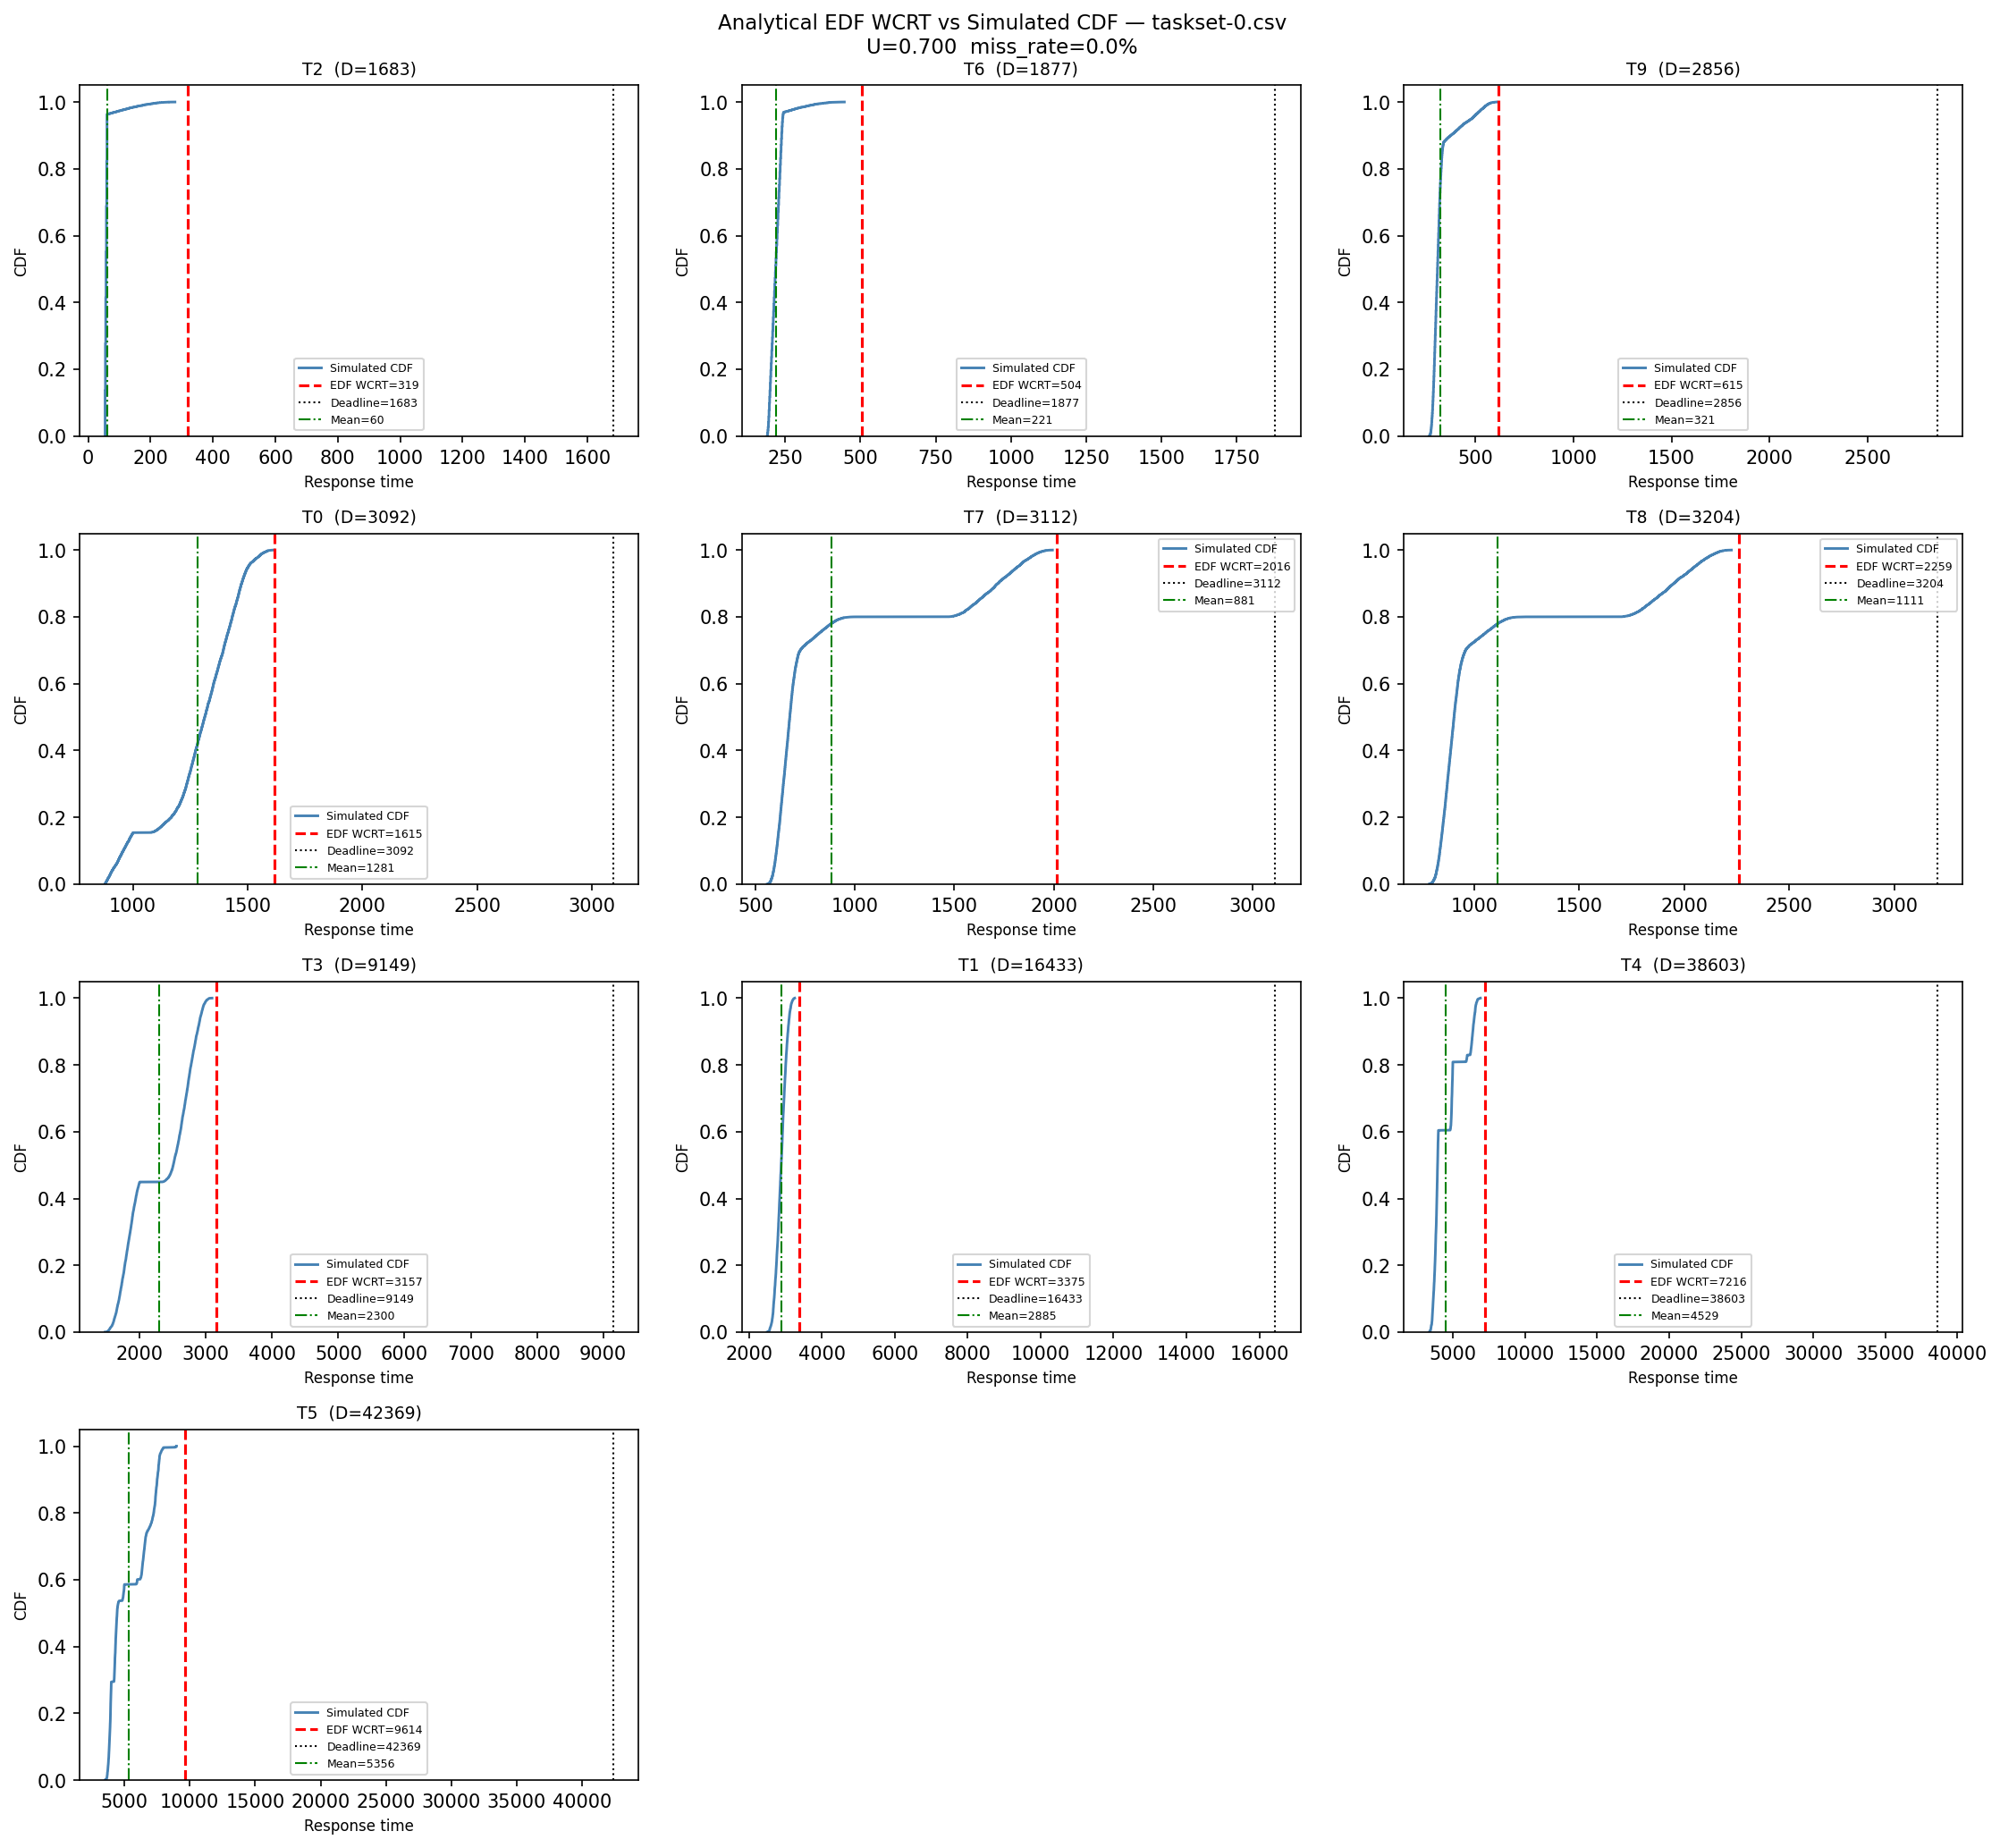
\includegraphics[width=\textwidth]{figures/harmonic/cdf_u70_taskset-0.png}
    \caption{Simulated CDF vs.\ EDF WCRT at $U \approx 0.70$, harmonic (taskset-0).}
    \label{fig:cdf_h_u70}
\end{minipage}\hfill
\begin{minipage}{0.48\textwidth}
    \centering
    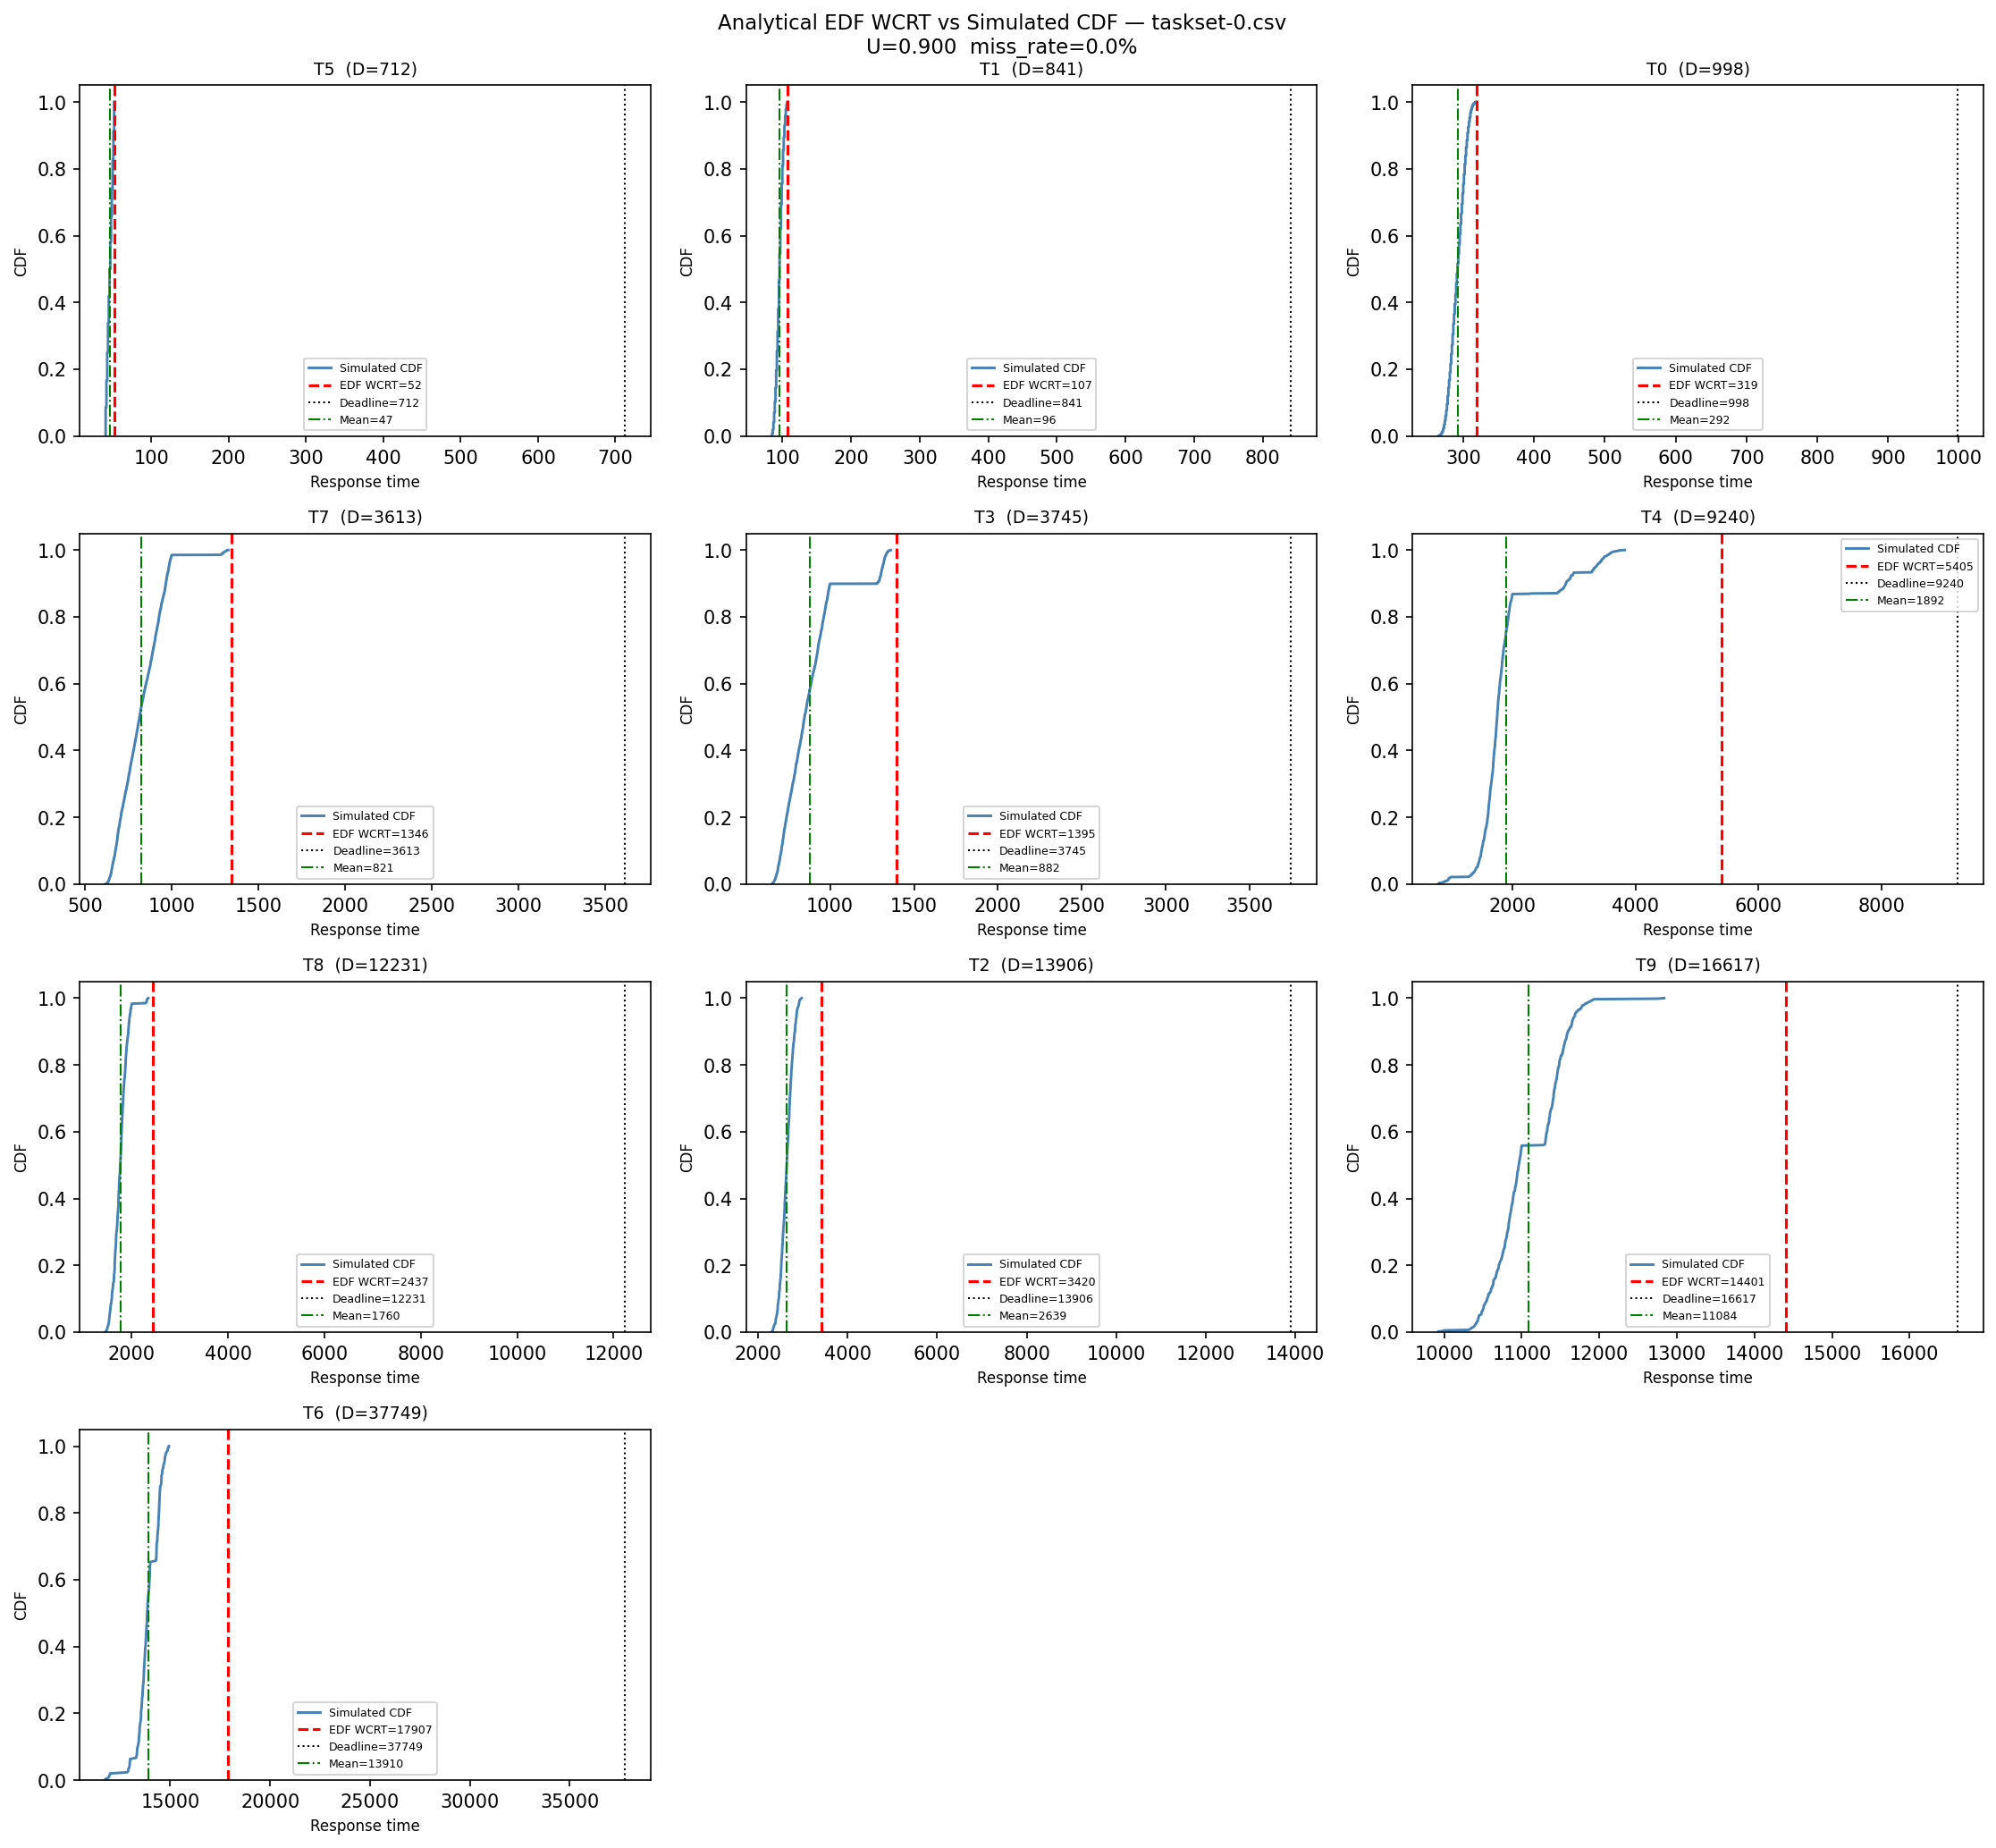
\includegraphics[width=\textwidth]{figures/harmonic/cdf_u90_taskset-0.png}
    \caption{Simulated CDF vs.\ EDF WCRT at $U \approx 0.90$, harmonic (taskset-0).}
    \label{fig:cdf_h_u90}
\end{minipage}
\end{figure}

% ─────────────────────────────────────────────────────────────────────────────
\section{Discussion}
\label{sec:discussion}
% ─────────────────────────────────────────────────────────────────────────────

\subsection{Why EDF Dominates at High Utilisation}

EDF achieves 100\% schedulability across all four utilisation levels because the Processor
Demand Criterion (Eq.~\ref{eq:pdc}) is both necessary and sufficient for synchronous
constrained-deadline task sets: any set with $U \leq 1$ that satisfies the demand bound is
provably schedulable. All 80 sets in our benchmark have $U < 1$, and none violated the demand
bound, so EDF passes unconditionally.

DM, by contrast, has no tight utilisation bound for constrained-deadline tasks. The sufficient
hyperbolic bound for $n = 10$ tasks is:
\[
    \prod_{i=1}^{n}\!\left(\frac{C_i}{T_i} + 1\right) \leq 2
    \;\Longrightarrow\; U \lesssim n\bigl(2^{1/n} - 1\bigr)
    \approx 10 \times 0.0718 = 0.718
\]
At utilisation $\approx 70\%$ all sets pass the hyperbolic bound; at $\approx 90\%$ it no
longer applies. Yet 18 of the 20 u90 sets still pass DM, because the RTA
(Eq.~\eqref{eq:rta}) is the exact, task-specific test---not a conservative utilisation
ceiling. The two failures arise from particular combinations of deadlines and periods that
cause cascading interference on the lowest-priority tasks, pushing their WCRTs beyond their
deadlines.

This demonstrates the theoretical result from Buttazzo~\cite{buttazzo2024}: EDF's optimality
becomes decisive as utilisation approaches 1, while DM schedulability depends critically on
the specific task parameters.

\subsection{Hyperperiod Explosion and the Harmonic Remedy}

A key practical finding from the primary benchmark is that 66 of the 80 task sets (82.5\%)
have hyperperiods too large to simulate---in several cases exceeding $10^{11}$ time units,
with total job counts reaching tens of billions. This arises because the generated task sets
use non-harmonic periods (no common small divisor), and $\mathrm{lcm}$ grows combinatorially
with non-harmonic integers.

Regenerating the benchmark with harmonic periods (Section~\ref{sec:harmonic}) eliminates
this problem entirely: all 80 harmonic sets are tractable and fully simulated. This confirms
that the hyperperiod explosion in the primary benchmark is a property of the period generation
strategy, not of the scheduling algorithms or utilisation levels themselves. The harmonic
results validate the PDC-only conclusions from the primary benchmark across all 80 sets,
and extend the Monte Carlo validation from 14 sets to the full benchmark.

\subsection{Pessimism of Analytical WCRT Bounds}

Across all 14 fully simulated sets, the observed maximum response time (over 300 Monte Carlo
runs, each with randomised execution times in $[B_i, C_i]$) was strictly below the analytical
WCRT in every case. The deadline miss rate was 0.0\% universally. The gap between the mean
observed response time and the analytical WCRT is substantial---typically the mean is at
30--60\% of the WCRT---because the WCRT assumes a simultaneous worst-case phasing of all job
releases (the critical instant), which is a rare event when execution times vary. The P95 and
P99 statistics cluster near the mean, confirming that the worst-case scenario almost never
materialises in stochastic operation.

% ─────────────────────────────────────────────────────────────────────────────
\section{Conclusion}
\label{sec:conclusion}
% ─────────────────────────────────────────────────────────────────────────────

As can be seen in Section~\ref{sec:results}, EDF reaches 100\% schedulability at all
utilisation levels, whereas DM only reaches 100\% schedulability at utilisation levels
30\%, 50\%, and 70\%, dropping down to 90\% schedulability at utilisation level 90\%.
The two task sets that DM failed to schedule confirm that above the hyperbolic bound,
DM does not guarantee schedulability. This confirms that in order to verify exact
schedulability for DM, RTA is necessary.

Our results in Section~\ref{sec:results} also confirm that when a stochastic Monte Carlo
simulation is run, all deadlines are met and the observed response time is lower than the
WCRT, confirming that the analytical bounds are correct although pessimistic.

Based on our results and analysis, we can conclude that at or below utilisation levels of
70\%, running DM is sufficient and most likely preferred, due to it being simpler to
implement with static priorities and no runtime overhead. With that in mind, implementing
EDF is necessary when the system must approach full CPU utilisation, as its dynamic
nature and provably schedulable guarantee for any utilisation level below or equal to
100\% make it a more reliable choice.

% ─────────────────────────────────────────────────────────────────────────────
\section{Limitations and Future Work}
\label{sec:limitations}
% ─────────────────────────────────────────────────────────────────────────────

\subsection{Limitations}

The analysis is restricted to a synchronous, independent, periodic task model on a
single uniprocessor with no shared resources or task dependencies, excluding
real-world concerns such as aperiodic tasks, priority inversion, and multi-core
execution. The benchmark is relatively small---20 synthetic task sets of 10 tasks
each per utilisation level---and the four discrete utilisation targets leave the
region where DM begins to fail poorly resolved.

A key practical bottleneck in the primary benchmark was hyperperiod explosion: 66 of 80
task sets exceeded the 200,000-job threshold, limiting exact EDF WCRT simulation to only
14 sets. The harmonic benchmark (Section~\ref{sec:harmonic}) resolves this entirely---all
80 harmonic sets are tractable---confirming that the issue is specific to the non-harmonic
period generation strategy rather than a fundamental limitation of the analysis.
Additionally, although the CSV task files contain release jitter values, the current
RTA treats jitter as zero; incorporating jitter into the interference term
$\lceil (R_i + J_j) / T_j \rceil \cdot C_j$ would yield more accurate WCRT bounds.
Finally, the stochastic simulation used 300 runs per task set, which is sufficient
to observe the distribution shape but may not provide tight estimates at the tail
(P99 and beyond).

\subsection{Future Work}

The harmonic benchmark resolves the tractability problem for simulation, but the primary
benchmark's non-harmonic sets still lack exact EDF WCRTs. Applying compositional EDF
WCRT bounds or busy-period window analysis would close this gap without requiring
harmonic periods, and would make the analysis applicable to arbitrary real-world period
distributions.

Incorporating release jitter into the RTA (replacing $\lceil R_i/T_j \rceil$ with
$\lceil (R_i + J_j)/T_j \rceil$) would improve accuracy and better reflect realistic
task activation behaviour, since the CSV files already contain jitter values that the
current analysis ignores. Increasing Monte Carlo runs from 300 to approximately 10,000
would yield statistically tighter P99 estimates. Finally, extending the framework to
multi-core platforms using partitioned or global EDF is a natural next step in the
distributed real-time systems context.

% ─────────────────────────────────────────────────────────────────────────────
\begin{thebibliography}{9}
\bibitem{buttazzo2024}
G.~C.~Buttazzo,
\textit{Hard Real-Time Computing Systems: Predictable Scheduling Algorithms and Applications},
4th ed.\ Springer, 2024.
\end{thebibliography}

\end{document}
